\chapter{Additional Examples}

\begin{example}
	\index{Example: Maximum likelihood}
	\emph{Consider a uniform distribution\index{Uniform distribution} centered on $0$ with width $2a$. The density distribution is given by $p(x|a)=\frac{\mathbb{I}(x\in[-a,a])}{2a}$.}
	
	\begin{enumerate}
		\item \emph{Given a dataset $x_1,x_2,\dots x_n$ what is the MLE estimate of $a$?}
		
		\begin{equation}
			\begin{split}
				p(D|a,I)&=\prod_{j=1}^n(\frac{\mathbb{I}(x_j\in[-a,a])}{2a})\\
				&=\frac{1}{(2a)^n} \text{ for $x_j\in [-a,a]$}
			\end{split}
		\end{equation}
		The likelihood cannot be optimized using the derivative approach since $\frac{d\ln(p(D|a,I))}{da}\big|_{a=\hat{a}_{\text{MLE}}}=0$ does not yield a useable result. Instead note that $(2a)^{-n}$ is a monotonic decreasing function of $a$, meaning the likelihood will be largest for the smallest value of $a$ whilst obeying $x_j\leq a$. This means $\hat{a}_{\text{MLE}}=\max(|x_1|,|x_2|,\dots |x_n|)$, since this will yield the smallest value of $a$ that is still larger or equal to all the data values.
		
		\item \emph{What probability would the model assign to a new datapoint $x_{n+1}$ using $\hat{a}_{\text{MLE}}$?}
		
		\begin{equation}
			p(x_{n+1}|D,I)|_{\text{MLE}} =\frac{1}{2\max(|x_1|,|x_2|,\dots |x_n|)}
		\end{equation}
		for $-\max(|x_1|,|x_2|,\dots |x_n|) \leq x_{n+1}\leq \max(|x_1|,|x_2|,\dots |x_n|)$.
		
		\item \emph{Do you see any problems with the above approach? Briefly suggest a better approach.}\newline
		
		The model place zero probability mass outside the training data. You need to use prior information.
	\end{enumerate}
\end{example}





\begin{example}
	\index{Example: Normal distribution}
	\emph{Suppose we have two sensors with unknown variances $\nu_1$ and $\nu_2$ ($\nu_1\neq \nu_2$), but unknown (and the same) mean, $\mu$. Suppose we observe $n_1$ observation from $y_i^{(1)}\sim N(y_i^{(1)}|\mu,\nu_1)$ from the first sensor and $y_i^{(2)}\sim N(y_i^{(2)}|\mu,\nu_2)$ from the second sensor. Let $D$ represent all the data from both sensors. What is the posterior $p(\mu|D,\nu_1,\nu_2,I)$, assuming a non-informative prior for $\mu$?}
	
	\begin{equation}
		p(\mu|D,\nu_1,\nu_2,I) =\frac{p(D|\mu,\nu_1,\nu_2,I)p(\mu|\nu_1,\nu_2,I)}{p(D|\nu_1,\nu_2,I)}
	\end{equation}
	with $p(\mu|\nu_1,\nu_2,I)=\text{Unif}(a,b)$ since it is supposed to be an uninformative prior. The likelihood 
	\begin{equation}
		\begin{split}
			p(D|\mu,\nu_1,\nu_2,I) &= \prod_{i=1}^{N^{(1)}}\frac{1}{\sqrt{2\pi \nu_1}}e^{-\frac{1}{2\nu_1}(y_i^{(1)}-\mu)^2}\prod_{j=1}^{N^{(2)}}\frac{1}{\sqrt{2\pi \nu_2}}e^{-\frac{1}{2\nu_2}(y_j^{(2)}-\mu)^2}\\
			& = (2\pi \nu_1)^{-\frac{N^{(1)}}{2}}(2\pi \nu_2)^{-\frac{N^{(2)}}{2}}e^{-\frac{1}{2\nu_1}\sum_{i=1}^{N^{(1)}}(y_i^{(1)}-\mu)^2-\frac{1}{2\nu_2}\sum_{j=1}^{N^{(2)}}(y_j^{(2)}-\mu)^2}\\
			&\propto e^{-\frac{1}{2\tilde{\nu}}(\mu-\tilde{\mu})^2},
		\end{split}
	\end{equation}
	where $\tilde{\nu}$ can be found by considering the part of the exponent for $-\frac{\mu^2}{2\tilde{\nu}}$ and then identifying $\tilde{\nu}$, yielding
	\begin{equation}
		\tilde{\nu}= \frac{1}{\frac{N^{(1)}}{\nu_1}+\frac{N^{(2)}}{\nu_2}}.
	\end{equation}
	Similarly by considering the part of the exponent for the double product
	\begin{equation}
		\tilde{\mu} = \tilde{\nu}\bigg(\frac{N^{(1)}\bar{y}^{(1)}}{\nu_1}+\frac{N^{(2)}\bar{y}^{(2)}}{\nu_2}\bigg).
	\end{equation}
\end{example}

\begin{example}
	\index{Example: Bayes naive classifier}
	\emph{Consider a $3$-class naive Bayes classifier\footnote{The naive Bayes classifier assume the class conditional density can be written as a product of one-dimensional densities~\citep[p.84]{murphy2013machine}} with one binary feature and one Gaussian feature $y\sim \text{Mu}(y|\pi,1)$, $x_1|y=c\sim \text{Ber}(x_1|\theta_c)$, $x_2|y=c\sim N(x_2|\mu_c,\sigma_c^2)$ with}
	\begin{equation}
		\begin{split}
			\pi = \begin{pmatrix}
				0.5 \\
				0.25 \\
				0.25
			\end{pmatrix}, 
			\theta = \begin{pmatrix}
				0.5 \\
				0.5 \\
				0.5
			\end{pmatrix}, 
			\mu = \begin{pmatrix}
				-1 \\
				0 \\
				1
			\end{pmatrix},
			\sigma^2 = \begin{pmatrix}
				1 \\
				1 \\
				1
			\end{pmatrix}
		\end{split}
	\end{equation}
	
	\begin{enumerate}
		\item \emph{Compute $p(y|x_1=0,x_2=0)$.}
		
		\begin{equation}
			\begin{split}
				p(y=c|x_1=0,x_2=0,I) & = \frac{p(x_1=0,x_2=0|y=c,I)p(y=c|I)}{p(x_1=0,x_2=0|I)}\\
				&= \frac{p(x_1=0|x_2=0,y=c,I)p(x_2=0|y=c,I)p(y=c|I)}{p(x_1=0,x_2=0|I)}\\
				&= \frac{p(x_1=0|y=c,I)p(x_2=0|y=c,I)p(y=c|I)}{p(x_1=0,x_2=0|I)}\\
				&= \frac{p(x_1=0|y=c,I)p(x_2=0|y=c,I)p(y=c|I)}{\sum_{c'} p(x_1=0|y=c',I)p(x_2=0|y=c',I)p(y=c'|I)}\\
			\end{split}
		\end{equation}
		with
		\begin{equation}
			\begin{split}
				p(x_1=0|y,I) &= \text{Ber}(x_1=0|\theta)\\
				&= \begin{pmatrix}
					0.5 \\ 0.5\\ 0.5
				\end{pmatrix}\\
				p(x_2=0|y,I) &= N(x_2=0|\mu,\sigma^2)\\
				&= \frac{1}{\sqrt{2\pi \sigma^2}}e^{-\frac{1}{2}(\frac{x_2-\mu}{\sigma})^2}\\
				&\simeq  \begin{pmatrix}
					0.24 \\ 0.4\\ 0.24
				\end{pmatrix}\\
				p(y|\pi) &= \pi\\
			\end{split}
		\end{equation}
		\begin{equation}
			p(y=c|x_1=0,x_2=0,I) = \begin{pmatrix}
				0.43 \\ 0.35\\ 0.22
			\end{pmatrix}
		\end{equation}
		
		\item \emph{Compute $p(y|x_1=0,I)$.}
		
		\begin{equation}
			\begin{split}
				p(y=c|x_1=0,I) & = \frac{p(x_1=0|y=c,I)p(y=c|I)}{p(x_1=0|I)}\\
				&= \frac{p(x_1=0|y=c,I)p(y=c|I)}{\sum_{c'}p(x_1=0|y=c',I)p(y=c'|I)}\\
				&= \pi\\
				& = \begin{pmatrix}
					0.5 \\ 0.25\\ 0.25
				\end{pmatrix}
			\end{split}
		\end{equation}
		
		\item \emph{Compute $p(y|x_2=0,I)$.}
		
		\begin{equation}
			\begin{split}
				p(y=c|x_2=0,I) & = \frac{p(x_2=0|y=c,I)p(y=c|I)}{p(x_2=0|I)}\\
				&= \frac{p(x_2=0|y=c,I)p(y=c|I)}{\sum_{c'}p(x_2=0|y=c',I)p(y=c'|I)}\\
				& = \begin{pmatrix}
					0.43 \\ 0.35\\ 0.22
				\end{pmatrix}
			\end{split}
		\end{equation}
		
		\item \emph{Explain any interesting patterns you see in your results.} \newline
		
		Since $\theta_c=\theta_j\forall c,j\in \{c\}$ the prior information is propagated through in calculating $p(y|x_1=0,I)$ and $x_1$ does not impact $p(y|x_1=0,x_2=0,I)$, as can be seen by comparing $p(y|x_1=0,x_2=0,I)$ and $p(y|x_2=0,I)$. This can be seen by considering
		\begin{equation}
			\begin{split}
				p(y=c|x_1=0,x_2=0,I) & = \frac{p(x_1=0|y=c,I)p(x_2=0|y=c,I)p(y=c|I)}{\sum_{c'}p(x_1=0|y=c',I)p(x_2=0|y=c',I)p(y=c'|I)}\\
				& = \frac{p(x_2=0|y=c,I)p(y=c|I)}{\sum_{c'}p(x_2=0|y=c',I)p(y=c'|I)}\\
				& = p(y=c|x_2=0,I)
			\end{split}
		\end{equation}
		where it has been used that $p(x_1=0|y=c,I) = p(x_1=0|y=c',I)\forall c,c'\in \{c\}$ for the second equality.
	\end{enumerate} 
\end{example}

\begin{example}
	\label{ex:313}
	\index{Example: Posterior predictive}
	\emph{The posterior predictive for a single multinomial trial with a Dirichlet prior is given by}
	\begin{equation}
		\begin{split}
			p(j|D,I) &= \int d\theta p(j,\theta|D,I)\\
			&= \int d\theta p(j|\theta,D,I)p(\theta|D,I)\\
			&= \int d\theta_j p(j|\theta_j,I)\bigg(\int d\theta_{-j} p(\theta_{-j},\theta_j|D,I)\bigg)\\
			&= \int d\theta_j p(j|\theta_j,I)p(\theta_j|D,I)\\
			& = \mathbb{E}[\theta_j|D,I]\\
			& = \frac{\alpha_{j}+N_j}{\sum_k(\alpha_k+N_k)}\\
			& = \frac{\alpha_{j}+N_j}{\alpha_0+N_0}\\
		\end{split}
	\end{equation}
	\emph{where $\theta_{-j}= \theta \backslash \theta_j$. Now consider predicting a batch of new data, $\tilde{D}=\{x_1,x_2,\dots x_m\}$, consisting of $m$ single multinomial trials (think of predicting the next $m$ words in a sentence, assuming they are drawn iid). Derive an expression for $p(\tilde{D}|D,\alpha,I)$. Your answer should be a function of $\alpha$, and the new counts (sufficient statistics) defined as}
	\begin{equation}
		\begin{split}
			N_k^{\text{old}} & = \sum_{i\in D} \mathbb{I}(x_i=k),\\
			N_k^{\text{new}} & = \sum_{i\in \tilde{D}} \mathbb{I}(x_i=k)\\
		\end{split}
	\end{equation}
	
	\begin{equation}
		\begin{split}
			p(\tilde{D}|D,\alpha,I) & = \int d\theta p(\tilde{D},\theta|D,\alpha,I) \\ 
			& = \int d\theta p(\tilde{D}|\theta,\alpha,I)p(\theta|D,\alpha,I) \\
			&=\int d\theta \text{Mu}(x_1,x_2,\dots |\theta)\text{Dir}(\theta|N_1^{\text{old}}+\alpha_1,N_2^{\text{old}}+\alpha_2,\dots)\\
			&= \begin{pmatrix}
				N^{\text{new}}!\\
				\prod_k N_k^{\text{new}}!
			\end{pmatrix}\frac{B(\alpha+N^{\text{old}}+N^{\text{new}})}{B(\alpha+N^{\text{old}})}
		\end{split}
	\end{equation}
	where $\begin{pmatrix}
		N^{\text{new}}!\\
		\prod_k N_k^{\text{new}}!
	\end{pmatrix}$ is the binomial coefficient.	In the case of a one hot encoding of classes, the multinomial coefficient equals unity. In the case of a $m=1$, then
	\begin{equation}
		\begin{split}
			p(\tilde{D}=j|D,\alpha,I) &= \begin{pmatrix}
				N^{\text{new}}!\\
				N^{\text{new}}!
			\end{pmatrix}\frac{B(\alpha+N^{\text{old}}+1)}{B(\alpha+N^{\text{old}})}\\
			&=\frac{\Gamma(\alpha_j+N^{\text{old}}_j+1)}{\Gamma(\alpha+N^{\text{old}}+1)}\frac{\Gamma(\alpha_j+N^{\text{old}}_j)}{\Gamma(\alpha+N^{\text{old}})}\\
			&=\frac{\alpha_j+N^{\text{old}}_j}{\alpha+N^{\text{old}}}\\
		\end{split}
	\end{equation}
	which is the result given in the exercise.
	
\end{example}

\begin{example}
	
	\begin{enumerate}
		\index{Example: Posterior predictive}
		\item \emph{Suppose we compute the empirical distribution over letters of the Roman alphabet plus the space character (a distribution over $27$ values) from $2000$ samples. Suppose we see the letter "e" $260$ times. What is $p(x_{201}=\text{e}|D)$? Assume $\theta\sim \text{Dir}(\alpha_1,\dots \alpha_{27})$, where $\alpha_k=10\forall k$.}\newline
		
		As shown in example \ref{ex:313}
		\begin{equation}
			\begin{split}
				p(x_{2001}=\text{e}|D) & =\frac{\alpha_{5}+N_5}{\alpha_0+N_0}\\
				&= \frac{10+260}{10\cdot 27+2000}\\
				&\simeq 0.12
			\end{split}
		\end{equation}
		
		\item \emph{Suppose, in thge $2000$ samples, we saw "e" $260$ times, "a" $100$ times and "p" $87$ times. What is $p(x_{2001}=\text{p},x_{2002}=\text{a}|D)$ if we assume $\theta\sim \text{Dir}(\alpha_1,\dots \alpha_{27})$, where $\alpha_k=10\forall k$?}\newline
		
		\begin{equation}
			\begin{split}
				p(x_{2001}=\text{p},x_{2002}=\text{a}|D) & = p(x_{2001}=\text{p}|D,x_{2002}=\text{a})p(x_{2002}=\text{a}|D)\\
				&=p(x_{2001}=\text{p}|D)p(x_{2002}=\text{a}|D)\\
				&=\frac{10+87}{10\cdot 27+2000}\frac{10+100}{10\cdot 27+2001}\\
				&\simeq 0.002
			\end{split}
		\end{equation}
	\end{enumerate}
	
\end{example}


\begin{example}
	\index{Example: Posterior odds}
	\index{Example: Posterior mean}
	\emph{Let $x_{iw}=1$ if word "w" occurs in document "i" and $x_{iw}=0$ otherwise. Let $\theta_{cw}$ be the probability that word "w" occurs in document of class "c". Then the log-likelihood that document $x$ belong to class "c" is given by}
	\begin{equation}
		\begin{split}
			\ln(p(x_i|c,\theta,I))&=\ln\bigg(\prod_{w=1}^{W}\theta_{cw}^{x_{iw}}(1-\theta_{cw})^{1-x_{iw}}\bigg)\\
			&= \sum_{w=1}^{W}[x_{iw}\ln(\theta_{cw})+(1-x_{iw})\ln(1-\theta_{cw})]\\
			&= \sum_{w=1}^{W}[x_{iw}\ln(\frac{\theta_{cw}}{1-\theta_{cw}})+\ln(1-\theta_{cw})]\\
		\end{split}
	\end{equation}
	\emph{where W is the number of words in the vocabulary. We can write this more succinctly as}
	\begin{equation}
		\ln(p(x_i|c,\theta,I))=\phi(x_i)^T\beta_c,
	\end{equation}
	\emph{where $x_i = (x_{i1},\dots x_{iw})$ is a bit vector, $\phi(x_i)=(x_i, 1)$ and}
	\begin{equation}
		\beta_c = \begin{pmatrix}
			\ln(\frac{\theta_{c1}}{1-\theta_{c1}}) & \dots & \ln(\frac{\theta_{cw}}{1-\theta_{cw}}) & \sum_{w=1}^{W} \ln(1-\theta_{cw})
		\end{pmatrix}^T
	\end{equation}
	\emph{we see that this is a linear classifier, since the class conditional density is a linear function of the parameters $\beta_c$.}
	\begin{enumerate}
		\item \emph{Assuming $p(c=1)=p(c=2)=\frac{1}{2}$, write down an expression for the log posterior odds ratio $\log_2(\frac{p(c=1|x_i)}{p(c=2|x_i)})$ in terms  of the features $\phi(x_i)$ and the parameters, $\beta_1$ and $\beta_2$.}
		\begin{equation}
			p(c=j|x_i) = \frac{p(x_i|c_j)p(c=j)}{p(x_i)}\Rightarrow \log_2(\frac{p(c=1|x_i)}{p(c=2|x_i)}) = \log_2(\frac{p(x_i|c=1)}{p(x_i|c=2)}) = \phi(x_i)^T(\beta_1-\beta_2)
		\end{equation}
		
		\item \emph{Intuitively,words that occur in both classes are not very "discriminative" and therefore should not affect our beliefs about the class label. Consider a particular word, $\tilde{w}$. State the conditions on $\theta_{1,\tilde{w}}$ and $\theta_{2,\tilde{w}}$ (or equivalently $\beta_{1,\tilde{w}}$ or $\beta_{2,\tilde{w}}$) under which the presence or absence of $\tilde{w}$ in a test document will have no effect on the class posterior (such a word will be ignored by the classifier)}\newline
		
		In order fo redundant words to not influence the classification, they should contribute equally to the likelihood of each class. In that case $\beta_{1,\tilde{w}}=\beta_{2,\tilde{w}}$.
		
		\item \emph{The posterior mean etimate of $\theta$, using $\theta \sim \text{Beta}(\theta|\alpha=1,\beta=1)$ as a prior, is given by}
		\begin{equation}
			\mathbb{E}[\theta_{cw}|D,I] = \frac{1+\sum_{i\in c} x_{iw}}{2+n_c},
		\end{equation}
		\emph{where the sum is over $n_c$ documents in class "c". Consider a particular word, $\tilde{w}$, and suppose it always occurs in every document (regardless of class). Let there be $n_1$ documents of class $1$ and $n_2$ documents of class $2$, where $n_1\neq n_2$ in general. If we use the above mean value for $\theta_{cw}$, will word $\tilde{w}$ be ignored by our classifier? Explain.}\newline
		
		Recall $x_{i\tilde{w}}$ is a bit vector which is $1$ if word $\tilde{w}$ occurs in document "i". It is assumed $\tilde{w}$ occurs in all documents, so
		\begin{equation}
			\begin{split}
				\mathbb{E}[\theta_{1\tilde{w}}|D,I] &= \frac{1+n_1}{2+n_1}, \\ 
				\mathbb{E}[\theta_{1\tilde{w}}|D,I] &= \frac{1+n_2}{2+n_2}. \\ 
			\end{split}
		\end{equation}
		$n_1\neq n_2 \Leftrightarrow \mathbb{E}[\theta_{1\tilde{w}}|D,I] \neq \mathbb{E}[\theta_{2\tilde{w}}|D,I]$ in general, meaning the probability varies among classes (which is what we do not want). However, intuitively, this must be the case since it cannot be known if a word will be present in all documents without having seen all documents. Hence, the more documents a word has been observed in, the more precisely the probability of observing the word ($\theta$) can be estimated -- As should be the case. Indeed for the number of documents a word has been observed in going to inifity ($n_1,n_2\rightarrow \infty$) the expectation values approach equality -- As desired. Hence, the dynamics are as they should be; there is no undesired behavoir. The Author of the exercise see an issue with the potential difference in expectation values for a small number of documents because the Author has a large bias towards towards the word existing in all documents. This kind of information should enter the calculations as a dominating prior. Doing this will add an artificial number of documents from the prior and taking this number to go to infinity, or whatever represents the bias, will fix the supposed issue even for a small number of observed documents.
		
		\item \emph{What other ways can you think of whih encourage "irrelevant" words to be ignored?}\newline
		
		I can see three ways to work around the supposed issue;
		i) use a dominating prior (as described in the previous bullet), ii) enforce an equal amount of documents in each class for training data or iii) delete words that occur in all documents.
	\end{enumerate}
	
\end{example}

\begin{example}
	\index{Example: Naive Bayes}
	\emph{Consider a naive Bayes model (multivariate Bernoulli version) for spam classification with the vocabulary}
	\begin{equation}
		V = \{\text{secrete, offer, low, price, valued, customer, today, dollar, million, sports, is, for , play, healthy, pizza}\}
	\end{equation}
	\emph{and the following examples of messages}
	
	\begin{center}
		\begin{tabular}{ |c | c | }
			\hline
			Message & Class  \\
			\hline
			million dollar offer & spam  \\
			secret offer today & spam  \\
			secret is secret & spam \\
			low price for valued customer & ham \\
			play secret sports today & ham \\
			sports is healthy & ham \\
			low price pizza & ham \\
			\hline
		\end{tabular}
	\end{center}
	
	\emph{Give the MLE's for the following parameters: $\theta_{\text{spam}}, \theta_{\text{secret|spam}}, \theta_{\text{secret|ham}}, \theta_{\text{sports|ham}}, \theta_{\text{dollar|spam}}$.}\newline
	
	From \citep[p. 85]{murphy2013machine} the MLE estimator is given by the number of sentences with a given word divided by the total number of sentences, meaning
	\begin{equation}
		\begin{split}
			\hat{\theta}_{\text{spam}} & = \frac{N_{\text{spam}}}{N} = \frac{3}{7}\\
			\hat{\theta}_{\text{secret|spam}} & = \frac{N_{\text{secret|spam}}}{N_{\text{spam}}} = \frac{2}{3}\\
			\hat{\theta}_{\text{secret|ham}} & = \frac{N_{\text{secret|ham}}}{N_{\text{ham}}} = \frac{1}{4}\\
			\hat{\theta}_{\text{sports|ham}} & = \frac{N_{\text{sports|ham}}}{N_{\text{ham}}} = \frac{2}{4}\\
			\hat{\theta}_{\text{dollar|spam}} & = \frac{N_{\text{dollar|spam}}}{N_{\text{spam}}} = \frac{1}{3}\\
		\end{split}
	\end{equation}
\end{example}



\begin{example}
	\index{Example: Normal distribution}
	\emph{Prove that $(2\pi)^\frac{d}{2}|\Sigma|^{\frac{1}{2}}=\int dx e^{-\frac{1}{2}(x-\mu)^T\Sigma^{-1}(x-\mu)}$ for a d-dimensional Gaussian.}
	
	\begin{equation}
		\begin{split}
			(x-\mu)^T\Sigma^{-1}(x-\mu) & = (x-\mu)^T(Q\Lambda Q^{-1})^{-1}(x-\mu)\\
			&= (x-\mu)^TQ\Lambda^{-1}Q^{-1}(x-\mu)\\
		\end{split}
	\end{equation}
	where $\Sigma= Q\Lambda Q^{-1}$ is an eigen decomposition of $\Sigma$ with $Q$ being an orthonormal matrix and $\Lambda$ a diagonal matrix with the eigenvalues, $\lambda_i$. Now, let $y\equiv Q(x-\mu)$ then
	\begin{equation}
		\int dx e^{-\frac{1}{2}(x-\mu)^T\Sigma^{-1}(x-\mu)} = \int dy \bigg|\frac{dx}{dy}\bigg|e^{-\frac{1}{2}y^T\Lambda^{-1}y}.
	\end{equation}
	$x=Q^{-1}y+\mu\Rightarrow \frac{dx}{dy}=Q^{-1}$. $|Q^{-1}|=\frac{1}{|Q|}=1$ since $Q$ is orthonormal, meaning
	\begin{equation}
		\begin{split}
			\int dx e^{-\frac{1}{2}(x-\mu)^T\Sigma^{-1}(x-\mu)} &= \int dy e^{-\frac{1}{2}y^T\Lambda^{-1}y}\\
			&= \int dy e^{-\frac{1}{2}\sum_i\frac{y_i^2}{\lambda_i}}\\
			&= \prod_i\int dy e^{-\frac{1}{2}\frac{y_i^2}{\lambda_i}}\\
			& = \prod_i \sqrt{2\pi \lambda_i}\\
			& = (2\pi)^\frac{d}{2}(\prod_i\lambda_i)^\frac{1}{2}\\
			& = (2\pi)^\frac{d}{2}|\Sigma|^{\frac{1}{2}}
		\end{split}
	\end{equation}
	where for the last equality it has been used that $\prod_i\lambda_i=|\Sigma|$.
\end{example}
\begin{example}
	\label{eq:qwe}
	\index{Example: Normal distribution}
	\emph{Let $x\sim N(x|\mu,\Sigma)$ with $x\in \mathbb{R}^2$ meaning $x=\begin{pmatrix}
			x_1 & x_2
		\end{pmatrix}^T$ and $\mu=\begin{pmatrix}
			\mu_1 & \mu_2
		\end{pmatrix}^T$ and }
	\begin{equation}
		\Sigma=\begin{pmatrix}
			\sigma_1^2 &  \rho\sigma_1\sigma_2 \\
			\rho\sigma_1\sigma_2 & \sigma_2^2\\
		\end{pmatrix}
	\end{equation}
	\emph{where $\rho$ is the correlation coefficient. Write down $p(x_1,x_2)$.}
	
	\begin{equation}
		p(x_1,x_2)=\frac{1}{\sqrt{(2\pi)^d|\Sigma|}}e^{-\frac{1}{2}(x-\mu)^T\Sigma^{-1}(x-\mu)}
	\end{equation}
	with $d=2$ and the given $\Sigma$
	\begin{equation}
		\begin{split}
			\sqrt{(2\pi)^d|\Sigma|}&= \sqrt{(2\pi)^2(\sigma_1^2\sigma_2^2-\rho^2\sigma_1^2\sigma_2^2)}\\
			&= 2\pi \sigma_1\sigma_2\sqrt{1-\rho^2}.
		\end{split}
	\end{equation}
	\begin{equation}
		\Sigma^{-1}=\frac{1}{\rho^2-1}\begin{pmatrix}
			-\frac{1}{\sigma_1^2} & \frac{\rho}{\sigma_1\sigma_2}\\
			\frac{\rho}{\sigma_1\sigma_2} & -\frac{1}{\sigma_2^2}
		\end{pmatrix}
	\end{equation}
	\begin{equation}
		\begin{split}
			(x-\mu)^T\Sigma^{-1}(x-\mu) & = \begin{pmatrix}
				x_1-\mu_1 & x_2-\mu_2
			\end{pmatrix}\frac{1}{\rho^2-1}\begin{pmatrix}
				-\frac{1}{\sigma_1^2} & \frac{\rho}{\sigma_1\sigma_2}\\
				\frac{\rho}{\sigma_1\sigma_2} & -\frac{1}{\sigma_2^2}
			\end{pmatrix}\begin{pmatrix}
				x_1-\mu_1 \\ x_2-\mu_2
			\end{pmatrix}\\
			&= \frac{1}{\rho^2-1}\bigg[\bigg(\frac{x_1-\mu_1}{\sigma_1}\bigg)^2+\bigg(\frac{x_2-\mu_2}{\sigma_2}\bigg)^2-2\rho\frac{(x_1-\mu_1)(x_2-\mu_2)}{\sigma_1\sigma_2}\bigg]
		\end{split}
	\end{equation}
\end{example}

\begin{example}
	\index{Example: Normal distribution}
	\emph{Suppose we have two sensors with unknown variances $\nu_1$ and $\nu_2$ ($\nu_1\neq \nu_2$), but unknown (and the same) mean, $\mu$. Suppose we observe $n_1$ observation from $y_i^{(1)}\sim N(y_i^{(1)}|\mu,\nu_1)$ from the first sensor and $y_i^{(2)}\sim N(y_i^{(2)}|\mu,\nu_2)$ from the second sensor. Let $D$ represent all the data from both sensors. What is the posterior $p(\mu|D,\nu_1,\nu_2,I)$, assuming a non-informative prior for $\mu$?}
	
	\begin{equation}
		p(\mu|D,\nu_1,\nu_2,I) =\frac{p(D|\mu,\nu_1,\nu_2,I)p(\mu|\nu_1,\nu_2,I)}{p(D|\nu_1,\nu_2,I)}
	\end{equation}
	with $p(\mu|\nu_1,\nu_2,I)=\text{Unif}(a,b)$ since it is supposed to be an uninformative prior. The likelihood 
	\begin{equation}
		\begin{split}
			p(D|\mu,\nu_1,\nu_2,I) &= \prod_{i=1}^{N^{(1)}}\frac{1}{\sqrt{2\pi \nu_1}}e^{-\frac{1}{2\nu_1}(y_i^{(1)}-\mu)^2}\prod_{j=1}^{N^{(2)}}\frac{1}{\sqrt{2\pi \nu_2}}e^{-\frac{1}{2\nu_2}(y_j^{(2)}-\mu)^2}\\
			& = (2\pi \nu_1)^{-\frac{N^{(1)}}{2}}(2\pi \nu_2)^{-\frac{N^{(2)}}{2}}e^{-\frac{1}{2\nu_1}\sum_{i=1}^{N^{(1)}}(y_i^{(1)}-\mu)^2-\frac{1}{2\nu_2}\sum_{j=1}^{N^{(2)}}(y_j^{(2)}-\mu)^2}\\
			&\propto e^{-\frac{1}{2\tilde{\nu}}(\mu-\tilde{\mu})^2},
		\end{split}
	\end{equation}
	where $\tilde{\nu}$ can be found by considering the part of the exponent for $-\frac{\mu^2}{2\tilde{\nu}}$ and then identifying $\tilde{\nu}$, yielding
	\begin{equation}
		\tilde{\nu}= \frac{1}{\frac{N^{(1)}}{\nu_1}+\frac{N^{(2)}}{\nu_2}}.
	\end{equation}
	Similarly by considering the part of the exponent for the double product
	\begin{equation}
		\tilde{\mu} = \tilde{\nu}\bigg(\frac{N^{(1)}\bar{y}^{(1)}}{\nu_1}+\frac{N^{(2)}\bar{y}^{(2)}}{\nu_2}\bigg).
	\end{equation}
\end{example}

\begin{example}
	\index{Example: Bayes naive classifier}
	\emph{Consider a $3$-class naive Bayes classifier\footnote{The naive Bayes classifier assume the class conditional density can be written as a product of one-dimensional densities~\citep[p.84]{murphy2013machine}} with one binary feature and one Gaussian feature $y\sim \text{Mu}(y|\pi,1)$, $x_1|y=c\sim \text{Ber}(x_1|\theta_c)$, $x_2|y=c\sim N(x_2|\mu_c,\sigma_c^2)$ with}
	\begin{equation}
		\begin{split}
			\pi = \begin{pmatrix}
				0.5 \\
				0.25 \\
				0.25
			\end{pmatrix}, 
			\theta = \begin{pmatrix}
				0.5 \\
				0.5 \\
				0.5
			\end{pmatrix}, 
			\mu = \begin{pmatrix}
				-1 \\
				0 \\
				1
			\end{pmatrix},
			\sigma^2 = \begin{pmatrix}
				1 \\
				1 \\
				1
			\end{pmatrix}
		\end{split}
	\end{equation}
	
	\begin{enumerate}
		\item \emph{Compute $p(y|x_1=0,x_2=0)$.}
		
		\begin{equation}
			\begin{split}
				p(y=c|x_1=0,x_2=0,I) & = \frac{p(x_1=0,x_2=0|y=c,I)p(y=c|I)}{p(x_1=0,x_2=0|I)}\\
				&= \frac{p(x_1=0|x_2=0,y=c,I)p(x_2=0|y=c,I)p(y=c|I)}{p(x_1=0,x_2=0|I)}\\
				&= \frac{p(x_1=0|y=c,I)p(x_2=0|y=c,I)p(y=c|I)}{p(x_1=0,x_2=0|I)}\\
				&= \frac{p(x_1=0|y=c,I)p(x_2=0|y=c,I)p(y=c|I)}{\sum_{c'} p(x_1=0|y=c',I)p(x_2=0|y=c',I)p(y=c'|I)}\\
			\end{split}
		\end{equation}
		with
		\begin{equation}
			\begin{split}
				p(x_1=0|y,I) &= \text{Ber}(x_1=0|\theta)\\
				&= \begin{pmatrix}
					0.5 \\ 0.5\\ 0.5
				\end{pmatrix}\\
				p(x_2=0|y,I) &= N(x_2=0|\mu,\sigma^2)\\
				&= \frac{1}{\sqrt{2\pi \sigma^2}}e^{-\frac{1}{2}(\frac{x_2-\mu}{\sigma})^2}\\
				&\simeq  \begin{pmatrix}
					0.24 \\ 0.4\\ 0.24
				\end{pmatrix}\\
				p(y|\pi) &= \pi\\
			\end{split}
		\end{equation}
		\begin{equation}
			p(y=c|x_1=0,x_2=0,I) = \begin{pmatrix}
				0.43 \\ 0.35\\ 0.22
			\end{pmatrix}
		\end{equation}
		
		\item \emph{Compute $p(y|x_1=0,I)$.}
		
		\begin{equation}
			\begin{split}
				p(y=c|x_1=0,I) & = \frac{p(x_1=0|y=c,I)p(y=c|I)}{p(x_1=0|I)}\\
				&= \frac{p(x_1=0|y=c,I)p(y=c|I)}{\sum_{c'}p(x_1=0|y=c',I)p(y=c'|I)}\\
				&= \pi\\
				& = \begin{pmatrix}
					0.5 \\ 0.25\\ 0.25
				\end{pmatrix}
			\end{split}
		\end{equation}
		
		\item \emph{Compute $p(y|x_2=0,I)$.}
		
		\begin{equation}
			\begin{split}
				p(y=c|x_2=0,I) & = \frac{p(x_2=0|y=c,I)p(y=c|I)}{p(x_2=0|I)}\\
				&= \frac{p(x_2=0|y=c,I)p(y=c|I)}{\sum_{c'}p(x_2=0|y=c',I)p(y=c'|I)}\\
				& = \begin{pmatrix}
					0.43 \\ 0.35\\ 0.22
				\end{pmatrix}
			\end{split}
		\end{equation}
		
		\item \emph{Explain any interesting patterns you see in your results.} \newline
		
		Since $\theta_c=\theta_j\forall c,j\in \{c\}$ the prior information is propagated through in calculating $p(y|x_1=0,I)$ and $x_1$ does not impact $p(y|x_1=0,x_2=0,I)$, as can be seen by comparing $p(y|x_1=0,x_2=0,I)$ and $p(y|x_2=0,I)$. This can be seen by considering
		\begin{equation}
			\begin{split}
				p(y=c|x_1=0,x_2=0,I) & = \frac{p(x_1=0|y=c,I)p(x_2=0|y=c,I)p(y=c|I)}{\sum_{c'}p(x_1=0|y=c',I)p(x_2=0|y=c',I)p(y=c'|I)}\\
				& = \frac{p(x_2=0|y=c,I)p(y=c|I)}{\sum_{c'}p(x_2=0|y=c',I)p(y=c'|I)}\\
				& = p(y=c|x_2=0,I)
			\end{split}
		\end{equation}
		where it has been used that $p(x_1=0|y=c,I) = p(x_1=0|y=c',I)\forall c,c'\in \{c\}$ for the second equality.
	\end{enumerate} 
\end{example}

\begin{example}
	\index{Example: Posteroir median}
	\emph{Prove that the posterior median is the optimal estimate under L1 loss.}
	\begin{equation}
		\begin{split}
			\rho(\theta|D) &= \int_{-\infty}^\infty |x-\theta|p(x|D)dx\\
			&= \int_{-\infty}^{\theta} (x-\theta)p(x|D)dx+\int_{\theta}^\infty (\theta-x)p(x|D)dx\\
			& \Downarrow\\
			\frac{d \rho(\theta|D)}{d\theta}\bigg|_{\theta=\hat{\theta}} &= (\hat{\theta}-\hat{\theta})p(\hat{\theta}|D)+\int_{-\infty}^{\hat{\theta}} p(x|D)dx+(\hat{\theta}-\hat{\theta})p(\hat{\theta}|D)-\int_{\hat{\theta}}^\infty p(x|D)dx\\
			&=0\\
			& \Downarrow\\
			\int_{-\infty}^{\hat{\theta}} p(x|D)dx &= \int_{\hat{\theta}}^\infty p(x|D)dx\\
			&= 1- \int_{-\infty}^{\hat{\theta}} p(x|D)dx\\
			&\Downarrow \\
			& \int_{-\infty}^{\hat{\theta}} p(x|D)dx = \frac{1}{2}
		\end{split}
	\end{equation}
	which is the definition of the median.

\end{example}

\begin{example}
	\index{Example: Bayes factor}
	Consider the case where $x \in [0,1]$ and the distirbution of $\tilde{x}_j$ follow a truncated (since the uncerainty $\delta x$ is symmetric about $x_j$) normal distribution\index{Normal distribution} with mean $x_j$ and uncertainty $\delta x_j$\label{ex:BF1}
	\begin{equation}
		p(x_j|A,\delta x_j, \tilde{x}_j, I) = \begin{cases}
			\frac{1}{\sqrt{2\pi}\delta x_j}e^{-\frac{1}{2}\big(\frac{x_j-\tilde{x}_j}{\delta x_j}\big)^2} & \text{for  } x_j\in [0,1]\\
			0 & \text{Otherwise} 
		\end{cases}.
	\end{equation} 
	Hereby
	\begin{equation}
		I = \prod_{j=1}^n\int p(x_j|A,\delta x_j, \tilde{x}_j, I)p(\tilde{x}_j|A,\theta,\delta x, I)p(\theta|A,\delta x^{(1:n)},I) d\tilde{x}_j d\theta,
	\end{equation}
	where
	\begin{equation}
		\begin{split}
			p(\theta|A,\delta x^{(1:n)},I)
			& =  p(\theta|A,I)
		\end{split}.
	\end{equation}
	A prerequisite for evaluating the integral is assigning probabilities $p(\theta|A,I)$ and $p(\tilde{x}_j|A,\theta,\delta x, I)$. $p(\theta|A,I)$ represents the prior belief about the parameters $\theta$ whereas $p(\tilde{x}_j|A,\theta,\delta x, I)$ has to capture the nature of the data given the hypothesis, parameters, uncertainty of $x$ and background information. 
	
	\paragraph{Gaussian Approximation:} As a first approximation to the scenario in example \ref{ex:BF1} the Gaussian approximation can be considered. In this approximation the limited support of $x$ is neglected and the distribution of $\kappa$ is assumed to be symmetric around a single peak defined by the mean $\mu$, standard deviation $\sigma$. Example \ref{ex:gauss} show how the Gaussian distribution can be derived from these assumptions using the principle of maximum entropy\index{Maximum entropy}, meaning\label{ex:gauss2}
	\begin{equation}
		p(\tilde{x}_j|A,\theta,\delta x, I) = \frac{1}{\sqrt{2\pi}\sigma}e^{-\frac{1}{2}\big(\frac{\tilde{x}_j-\mu}{\sigma}\big)^2}
	\end{equation}
	where $\theta = \{\sigma,\mu\}$. Since the Gaussian distribution is the conjugate prior distribution of the Gaussian distribution
	\begin{equation}
		\begin{split}
			p(x^{(1:n)}|A,\theta,\delta x^{(1:n)}, I) &\equiv \prod_{j=1}^{n}\int p(\tilde{x}_j|A,\theta,\delta x, I)p(x_j|A,\delta x_j, \tilde{x}_j, I)d \tilde{x}_j\\
			&= \prod_{j=1}^n\frac{1}{(\sigma+\delta x_j)\sqrt{2\pi}}e^{-\big(\frac{x_j-\mu}{\sqrt{2}(\sigma+\delta x_j)}\big)^2}
		\end{split}
		\label{likelihood1}
	\end{equation}
	in this case. Assuming a uniform prior on both the mean and standard deviation
	\begin{equation}
		p(\theta|A,I) = \frac{1}{(\mu_{max}-\mu_{min})(\sigma_{max}-\sigma_{min})}.
		\label{prior1}
	\end{equation}
	Using equations \eqref{prior1} and \eqref{likelihood1} the integral, $I$ can be written
	\begin{equation}
		I = \frac{\int \prod_{j\in x^{(1:n)}}\frac{1}{(\sigma+\delta x_j)\sqrt{2\pi}}e^{-\big(\frac{x_{j}-\mu}{\sqrt{2}(\sigma+\delta x_j)}\big)^2} d\mu d\sigma}{(\mu_{max}-\mu_{min})(\sigma_{max}-\sigma_{min})}.
	\end{equation}
	The likelihood can be evaluated numerically via importance sampling. Alternatively an analytical solution can be obtained by i) assuming $\delta x_j\ll \sigma$ and ii) Taylor expanding the logarithm of the likelihood around a maximum defined by $\mu_0,\sigma_0$~\citep{Sivia2006}
	\begin{equation}
		L = L(\mu_0,\sigma_0)-\frac{1}{2}\begin{bmatrix}
			\Delta\mu & \Delta\sigma
		\end{bmatrix}
		\begin{bmatrix}
			\alpha & \gamma\\
			\gamma & \beta \\
		\end{bmatrix}\begin{bmatrix}
			\Delta\mu\\ \Delta\sigma
		\end{bmatrix}
		+\mathcal{O}(\Delta\mu^2),
		\label{eq:li}
	\end{equation}
	where $\Delta \mu = \mu-\mu_0$ and $\Delta\sigma = \sigma-\sigma_0$. $\mu_0$ and $\sigma_0$ are determined from requiring $\frac{\partial L}{\partial \mu}=\frac{\partial L}{\partial \sigma}=0$
	\begin{equation}
		\begin{split}
			\mu_0 &= \frac{1}{\tilde{N}}\sum_{j}x_j,\\
			\sigma_0 &= \frac{1}{\tilde{N}}\sum_j(x_j-\mu_0)^2.
		\end{split}
		\label{eq:s}	
	\end{equation}
	$\alpha,\beta$ and $\gamma$ can be determined by evaluating the second order partial derivatives at the maximum
	\begin{equation}
		\begin{split}
			\alpha & = \frac{\tilde{N}}{\sigma_0^2}\\
			\beta & = 2\alpha\\
			\gamma & = 0.
		\end{split}
		\label{eq:a}
	\end{equation} 
	The results of equations \eqref{eq:li},\eqref{eq:s} and \eqref{eq:a} are understood to apply for all distributions.
	Hereby
	\begin{equation}
		\begin{split}
			I &\approx \frac{e^{L(\mu_0,\sigma_0)}\tilde{I}}{(\mu_{max}-\mu_{min})(\sigma_{max}-\sigma_{min})} \\
			&\approx \frac{e^{L(\mu_0,\sigma_0)}}{(\mu_{max}-\mu_{min})(\sigma_{max}-\sigma_{min})}\frac{2\pi}{\sqrt{\alpha\beta}}\\
			&=\frac{(\sigma_0 \sqrt{2\pi})^{2-\tilde{N}}e^{-\frac{\tilde{N}}{2}}}{\tilde{N}\sqrt{2}(\mu_{max}-\mu_{min})(\sigma_{max}-\sigma_{min})}
		\end{split}
	\end{equation}
	where
	\begin{equation}
		\tilde{I} = \int_{\mu_{min}}^{\mu_{max}}d\mu\int_{\sigma_{min}}^{\sigma_{max}}d\sigma e^{-\frac{1}{2}(\alpha\Delta\mu^2+\beta\Delta\sigma^2)}.
	\end{equation}
	The integrals related to hypothesis B are computed analogously yielding the Bayes factor
	\begin{equation}
		\begin{split}
			\rm BF &\sim  \frac{(\mu_{max}-\mu_{min})(\sigma_{max}-\sigma_{min})}{\pi \sqrt{2}}\frac{\tilde{N}_1\tilde{N}_2}{\tilde{N}}\frac{\sigma_0^{2-\tilde{N}}}{\sigma_{0,1}^{2-\tilde{N}_1}\sigma_{0,2}^{2-\tilde{N}_2}},
		\end{split}
	\end{equation}
	where the second index in $\sigma_{0,s}$ denotes the value of $s$.
	
	\paragraph{Beta Approximation:} The advantage of the Gaussian approximation in example \ref{ex:gauss2} is that it yields an analytical soltuion. The disadvantage is that it does not properly account for the support and possible morphology of the distribution of $x$. An improved approximation is to take the limited support of $x$ into account and allow for asymmetry in the distribution. Example \ref{ex:beta} show how the beta distribution can be derived from these assumptions using the principle of maximum entropy\index{Maximum entropy}, meaning\label{sec:beta}
	\begin{equation}
		p(\tilde{x}_j|A,\theta, I) = \frac{1}{B(\alpha,\beta)} \tilde{x}_j^{\alpha-1}(1-\tilde{x}_j)^{\beta-1}
		\label{eq:p2}
	\end{equation}
	where $\theta =\{\alpha,\beta\}$ and $B(\alpha,\beta)$ denotes the beta function. Assuming again a uniform prior on the parameters of the beta distribution ($\alpha,\beta$)
	\begin{equation}
		p(\theta|A,I) = \frac{1}{(\alpha_{max}-\alpha_{min})(\beta_{max}-\beta_{min})}.
		\label{prior2}
	\end{equation}
	Given equations \eqref{prior2} and \eqref{eq:p2} the integral, $I$, can be evaluated numerically via importance sampling. The dimensionality of the integral in $I$ is $n+2$, meaning the complexity is dominated by (and scale with) the dimensionality of data. For this reason, it is worth considering approximating $p(x^{(1:n)}|A,\theta,\delta x^{(1:n)}, I)$. In the case of the beta distribution 
	\begin{equation}
		p(x^{(1:n)}|A,\theta,\delta x^{(1:n)}, I) =\frac{1}{B(\alpha,\beta)^n}\prod_{j=1}^{n}\frac{I_1}{\sqrt{2\pi \delta} x_j}
		\label{likelihood2}
	\end{equation}
	with
	\begin{equation}
		I_1 = \int_0^1e^{-\frac{1}{2}\big(\frac{x_j-\tilde{x}_j}{\delta x_j}\big)^2+\ln(B(\alpha,\beta) p(\tilde{x}_j|A,\theta, I))}d\tilde{x}_j.
	\end{equation}
	The exponent\footnote{The reason why the exponent is expanded rather than the integrand itself is that the latter will allow for a negative value of the integral.} can be Taylor expanded
	\begin{equation}
		\begin{split}
			-\frac{1}{2}\big(\frac{x_j-\tilde{x}_j}{\delta x_j}\big)^2+\ln(B(\alpha,\beta) p(\tilde{x}_j|A,\theta, I)) = \sum_{i=0}^{1} a_i\Delta x_j^i+\mathcal{O}(\Delta x_j^2)
		\end{split}
	\end{equation}
	with $\Delta x_j \equiv \tilde{x}_j-x_j$ and
	\begin{equation}
		\begin{split}
			a_0 & = (\alpha-1)\ln(x_j)+(\beta-1)\ln(1-x_j),\\
			a_1 & = \frac{\alpha-1}{x_j}+\frac{\beta-1}{x_j-1}.\\
		\end{split}
	\end{equation}
	Hereby
	\begin{equation}
		\begin{split}
			I_1 &\approx e^{a_0-a_1x_j}\int_0^1e^{a_1\tilde{x}_j}d\tilde{x}_j\\
			&= \frac{e^{a_0-x_j a_1}(e^{a_1}-1)}{a_1}
		\end{split}
	\end{equation}
	and
	\begin{equation}
		p(x^{(1:n)}|A,\theta,\delta x^{(1:n)}, I) \approx\frac{1}{B(\alpha,\beta)^n}\prod_{j=1}^{n}\frac{1}{\sqrt{2\pi \delta} x_j}\frac{e^{a_0-x_j a_1}(e^{a_1}-1)}{a_1}.
		\label{likelihood3}
	\end{equation}
\end{example}

\begin{example}
		\index{Example: Bayesian decision theory}
		\emph{Consider the following classic problem in decision theory/economics. Suppose you are trying to decide how much quantity, Q, of some product to buy to maximize your profits. The optimal amount will dependon how much demand, A, you think there is for the product, as well as its cost, C, and selling price, W. Suppose A is unknown but has a pdf f(A) and cdf F(A). We can evaluate the expected profit by ocnsidering two cases: If A>Q, then we seel all Q items, and make profit $\pi=(W-C)Q$; but if A<Q, we only sell A items, at profit $\pi=(W-C)A$, but have wasted $C(Q-A)$ on the unsold items. So the expected profit if we buy quantity, Q, is}
		\begin{equation}
			\mathbb{E}[\pi(Q)]=\int_{Q}^\infty dA (W-C)Qf(A)+\int_{0}^Q dA (W-C)Af(A)-\int_{0}^Q dA (Q-A)Cf(A).
		\end{equation}
		\emph{Simplify this equation, and then take derivatives with respect to $Q$ to show that the optimal quantity, $Q^*$, satisfies}
		\begin{equation}
			F(Q^*)=\frac{W-C}{W}.
		\end{equation}
		\begin{equation}
			\begin{split}
				\mathbb{E}[\pi(Q)] &= (W-C)Q(\cancelto{1}{F(\infty)}-F(Q))+(W-C)\int_{0}^Q dAAf(A)-CQ[F(Q)-\cancelto{0}{F(0)}]+C\int_{0}^Q dA Af(A)\\
				&= Q(W-C)-WQF(Q)+W\int_{0}^Q dA Af(A)
			\end{split}
		\end{equation}
		\begin{equation}
			\begin{split}
				\frac{d\mathbb{E}[\pi(Q)]}{dQ} = W-C-WF(Q)
			\end{split}
		\end{equation}
		Hence, $\frac{d\mathbb{E}[\pi(Q)]}{dQ}|_{q=Q^*}=0\rightarrow F(Q^*)=\frac{W-C}{W}$.
	\end{example}
	


\begin{example}
	\index{Example: Future event counts}
	\label{ex:events}
	Let $x=x_1+x_2+\dots x_M$ be the sum of future event counts and $y=\{y_1,y_2,y_3,\dots y_N\}$ be observed event counts. With this notation the expected\index{Expectation value} number of future events, $x$, and the associated uncertainty\index{Variance} can be written
	\begin{equation}
		\mathbb{E}[x|y,I]\pm \sqrt{\text{Var}[x|y,I]},
		\label{eq:mean_var}
	\end{equation}
	where
	\begin{equation}
		\begin{split}
			\mathbb{E}[x|y,I] &= \sum_i ip(x =i|y,I),\\
			\text{Var}[x|y,I] &=  \sum_i i^2p(x =i|y,I)-\mathbb{E}[x|y,I]^2.
		\end{split}
		\label{h1}
	\end{equation}
	The distribution over counts $p(x =i|y,I)$ can be expanded by marginalizing over a set of unknown parameters from underlying distributions. The details depend on the statistical assumptions imposed. In this example, different assumptions and their consequences will be investigated.
	
	\paragraph{Simple Poisson Assumption:} The most common assumption is to assume data follow a Poisson distribution\index{Poisson distribution} with an unknown rate parameter which will then be marginalized\index{Marginalized} over. An abvious choice of prior would be the conjugate gamma distribution\index{Gamma distribution} (which is also the distribution with maximum entropy\index{Maximum entropy}) with parameters $\alpha, \beta$, meaning
	\begin{equation}
		\begin{split}
			p(x =i|y,\alpha, \beta,I) &= \int d\lambda p(x =i,\lambda|y,\alpha, \beta,I)\\
			&=\int d\lambda p(x =i|\lambda,\alpha, \beta,y,I)p(\lambda|\alpha, \beta,y,I)\\
			&= \int d\lambda p(x =i|\lambda,\alpha, \beta,y,I)\frac{p(y|\lambda,\alpha, \beta,I)p(\lambda|\alpha, \beta,I)}{p(y|\alpha, \beta,I)}.
		\end{split}
		\label{h4}
	\end{equation}
	with
	\begin{equation}
		\begin{split}
			p(y|\alpha, \beta,I) & = \int d \lambda p(y|\alpha, \beta,\lambda,I)p(\lambda|\alpha, \beta,I),\\
			p(y|\alpha, \beta,\lambda,I) &= \prod_{j=1}^N\text{Poi}(y_j|\lambda)\\
			&= \lambda^{N\bar{y}}e^{-N\lambda}\prod_{j=1}^N \frac{1}{y_j!},\\
			p(\lambda|\alpha,\beta,I) &= \text{Ga}(\lambda|\alpha,\beta)\\ &=\frac{\beta ^\alpha}{\Gamma(\alpha)}\lambda^{\alpha-1}e^{-\beta \lambda}.
		\end{split}
	\end{equation}
	Meaning
	\begin{equation}
		p(y|\lambda,\alpha, \beta,I)p(\lambda|\alpha, \beta,I) = \frac{\beta^\alpha}{\Gamma(\alpha)}\lambda^{\alpha+N\bar{y}-1}e^{-(\beta+N)\lambda}\prod_{j=1}^N \frac{1}{y_j!}
	\end{equation}
	and consequently
	\begin{equation}
		\begin{split}
			\frac{p(y|\lambda,\alpha, \beta,I)p(\lambda|\alpha, \beta,I)}{p(y|\alpha, \beta,I)} &= \frac{\lambda^{\alpha+N\bar{y}-1}e^{-(\beta+N)\lambda}}{\int d\lambda \lambda^{\alpha+N\bar{y}-1}e^{-(\beta+N)\lambda}}\\
			&= \text{Ga}(\lambda|\alpha+N\bar{y},\beta+N)\\
		\end{split}
	\end{equation}
	Using that $p(x =i|\lambda,\alpha,\beta,y,I) = \text{Poi}(x =i|M\lambda)$ yields
	\begin{equation}
		\begin{split}
			\mathbb{E}[x|y,\alpha,\beta,I] &= \sum_ii\int d\lambda \text{Poi}(x = i|M\lambda)\text{Ga}(\lambda| \alpha+N\bar{y},\beta +N)\\
			&= M\int d\lambda\lambda\text{Ga}(\lambda | \alpha+N\bar{y},\beta +N)\\
			&= M \frac{\alpha+N\bar{y}}{\beta +N},
		\end{split}
	\end{equation}
	where for the second equality it has been used that $\sum_ii \text{Poi}(x = i|M\lambda)=M\lambda$ and for the second equality it has been realized that the second line denoted the expectation of a Gamma distribution with modified parameters. Similarly for the variance
	\begin{equation}
		\begin{split}
			\sum_i i^2p(x = i|y,\alpha,\beta,I) &=  \sum_ii^2\int d\lambda \text{Poi}(x =i|M\lambda)\text{Ga}(\lambda | \alpha+N\bar{y},\beta +N)\\
			&=M\int d\lambda (\lambda +M\lambda^2)\text{Ga}(\lambda|\alpha+N\bar{y},\beta +N)\\
			&=\mathbb{E}[x|y,\alpha,\beta,I]+M^2\int d\lambda \lambda^2\text{Ga}(\lambda|\alpha+N\bar{y},\beta +N)\\
			&=\mathbb{E}[x|y,\alpha,\beta,I]+M^2\frac{\alpha+N\bar{y}}{(\beta +N)^2}+\mathbb{E}[x|y,\alpha,\beta,I]^2\\
		\end{split}
		\label{h2}
	\end{equation}
	where for the second equality it has been used that $\sum_ii^2\text{Poi}(x = i|M\lambda)=\text{Var}[i|M\lambda]+\mathbb{E}[x|M\lambda]^2=M\lambda +M^2\lambda^2$ and similarly for the fourth equality. Combining equations \eqref{h1} and \eqref{h2}, the variance can be written
	\begin{equation}
		\begin{split}
			\text{Var}[x|y,\alpha,\beta,I] & = \mathbb{E}[x|y,\alpha,\beta,I]+M^2\frac{\alpha+N\bar{y}}{(\beta +N)^2}\\
			& = M\bigg(1+\frac{M}{\beta+N}\bigg)\frac{\alpha+N\bar{y}}{\beta +N}.\\
		\end{split}
	\end{equation}
	In the limit of $\beta,\alpha\rightarrow 0$ equation \eqref{eq:mean_var} become
	\begin{equation}
		\begin{split}
			\mathbb{E}[x|y,I]\pm \sqrt{\text{Var}[x|y,I]} & = \lim\limits_{\alpha,\beta\rightarrow 0}\big(\mathbb{E}[x|y,\alpha,\beta,I]\pm \sqrt{\text{Var}[x|y,\alpha,\beta,I]}\big)\\
			& = M\bar{y}\pm \sqrt{M\big(1+\frac{M}{N}\big)\bar{y}}.\\ 
		\end{split}
		\label{h3}
	\end{equation}
	Equation \eqref{h3} informs that the expected number of future events is equal to the mean number of observed events per day multiplied with the number of days -- That makes sense. The variance of equation \eqref{h3} is proportional to the square root of the observed mean event count, which is to be expected from a Poisson distribution. It means $\mathbb{E}[x|y,I]\gg \sqrt{\text{Var}[x|y,I]}$ for $\bar{y}\gg 1$ and hence that the uncertainty approaches a negligible quantity. This is a strong implicit statement which easily can be broken. This can for example happen if the number of events is expected to vary due to a rate parameter that changes every day due to underlying dynamics, e.g. weather conditions. 
	
	
	\paragraph{Advanced Poisson Assumption:} In the case where the rate parameter of the Poisson distribution\index{Poisson distribution} is expected to have significant time variance while retaining unimodality, it is more accurate to assume that each rate parameter is unique, but drawn from the same gamma distribution\index{Gamma distribution}, meaning
	\begin{equation}
		\begin{split}
			p(x = i|y,\xi,\zeta,I) &= \int d\{\lambda_x\}d\{\lambda_y\} d\alpha d\beta p(x = i,\{\lambda_x\},\{\lambda_y\} ,\alpha, \beta|y,\xi,\zeta,I)\\
			&=\int d\{\lambda_x\}d\{\lambda_y\}d\alpha d\beta p(x=i,\{\lambda_x\}|\alpha, \beta,y,\xi,\zeta,I)p(\{\lambda_y\},\alpha,\beta|y,\xi,\zeta,I),
		\end{split}
		\label{r1}
	\end{equation}
	where $\xi,\zeta$ are the parameters of the prior distributions, $d\{\lambda_x\} = d\lambda_{x_1}d\lambda_{x_2}\dots d\lambda_{x_M}$ and $d\{\lambda_y\}=d\lambda_{y_1}d\lambda_{y_2}\dots d\lambda_{y_N}$ and
	\begin{equation}
		\begin{split}
			p(x=i,\{\lambda_x\}|\alpha, \beta,y,\xi,\zeta,I) &= p(x=i|\{\lambda_x\},\alpha, \beta,y,I)p(\{\lambda_x\}|\alpha, \beta,I),\\
			p(\{\lambda_y\},\alpha,\beta|y,\xi,\zeta,I) & = \frac{p(y|\{\lambda_y\},\alpha, \beta,I)p(\{\lambda_y\}|\alpha, \beta,I)p(\alpha|\xi,I)p(\beta|\zeta,I)}{p(y|\xi,\zeta,I)}
		\end{split}
	\end{equation}
	with
	\begin{equation}
		\begin{split}
			p(y|\xi,\zeta,I) & = \int d\{\lambda_y\} d\alpha d\beta p(y|\{\lambda_y\},\alpha, \beta,I)p(\{\lambda_y\}|\alpha, \beta,I)p(\alpha|\xi,I)p(\beta|\zeta,I),\\
			p(y|\{\lambda_y\},\alpha, \beta,I)p(\{\lambda_y\}|\alpha, \beta,I) &= \prod_{j=1}^N\text{Poi}(y_j|\lambda_{y_j})\text{Ga}(\lambda_{y_j}|\alpha,\beta).\\
		\end{split}
	\end{equation}
	The integrals over gamma can be evaluated individually viz
	\begin{equation}
		\begin{split}
			p(y_i|\alpha,\beta,I) &= \int d \lambda_{y_i} \text{Poi}(y_j|\lambda_{y_j})\text{Ga}(\lambda_{y_j}|\alpha,\beta)\\
			& = \begin{pmatrix}
				y_j+\alpha-1\\
				y_j
			\end{pmatrix}
			\bigg(\frac{\beta}{\beta+1}\bigg)^{y_j}\bigg(\frac{1}{\beta +1}\bigg)^\alpha\\
			&= \text{NB}\bigg(y_j|\alpha,\frac{\beta}{\beta +1}\bigg),
		\end{split}
	\end{equation}
	where NB abbreviates the negative binomial distribution\index{Negative binomial distribution}. The sum of negative binomial random variables is another negative binomial random variable, such that
	\begin{equation}
		\int d\{\lambda_x\} p(x=i,\{\lambda_x\}|\alpha, \beta,y,I) = \text{NB}\bigg(x=i|M\alpha,\frac{\beta}{\beta +1}\bigg),
	\end{equation}
	meaning equation \eqref{r1} can be written
	\begin{equation}
		\begin{split}
			p(x = i|y,\xi,\zeta,I) &= \frac{1}{p(y|\xi,\zeta,I)}\int d\alpha d\beta \text{NB}\bigg(x=i|M\alpha,\frac{\beta}{\beta +1}\bigg)\prod_{j=1}^N\text{NB}\bigg(y_j|\alpha,\frac{\beta}{\beta +1}\bigg)p(\alpha|\xi,I)p(\beta|\zeta,I).
		\end{split}
		\label{r2}
	\end{equation}
	Using the principle of maximum\index{Maximum entropy}, entropy, the distributions for $\alpha$ and $\beta$ can be assigned gamma distributions
	\begin{equation}
		\begin{split}
			p(\alpha|\xi,I) & = p(\alpha|a,b,I)\\
			&= \text{Ga}(\alpha| a, b),\\
			p(\beta|\zeta,I) & = p(\beta|c,d,I)\\
			&= \text{Ga}(\alpha| c, d),\\
		\end{split}
	\end{equation}
	with $\xi = \{a,b\}$ and $\zeta = \{c,d\}$. With this setup, $\mathbb{E}[x|y,\xi,\zeta,I]\pm \sqrt{\text{Var}[x|y,\xi,\zeta,I]}$ can be evaluated numerically using numerical methods like e.g. Hamiltonian Monte Carlo (see appendix \ref{app:HMC}). In this example, the pymc python packge~\citep{pymc} will be used (which utilize Hamiltonian Monte Carlo) with parameters $a=b=c=d =1$, corresponding to wide (low bias) gamma distributions. 
	
	\paragraph{Normal Assumption:} In case the distribution of $x$ is fairly symmetric around its peak and the summary statistics of equation \eqref{eq:mean_var} are the quantities of primary interest, a crude normal approximation can be made. For a continuous variable, equation \eqref{h1} become		
	\begin{equation}
		\begin{split}
			\mathbb{E}[x|y,I] &= \int xp(x|y,I),\\
			\text{Var}[x|y,I] &=  \int x^2p(x|y,I)-\mathbb{E}[x|y,I]^2.
		\end{split}
		\label{h1con}
	\end{equation}
	Assume $x$ is normally distributed\index{Normal distribution} with mean and precision $\mu\sim N(\mu|\text{mean}=\mu_0,\text{variance}=\frac{1}{c\tau})$ and $\tau\sim \text{Ga}(\tau|\alpha,\beta)$ following a normal and gamma distribution\index{Gamma distribution}, respectively. In this case
	\begin{equation}
		p(x|y,\mu_0,c,\alpha,\beta,I) = \int d\mu  d\tau p(x|\mu,\tau,y,I)\frac{p(y|\mu,\tau,I)p(\mu|\tau,\mu_0,c,I)p(\tau|\alpha,\beta,I)}{p(y|\mu_0,c,\alpha,\beta,I)}.
		\label{h6}
	\end{equation}
	With these assumptions, the likelihood is given by
	\begin{equation}
		\begin{split}
			p(y|\mu,\tau,I) &= \bigg(\frac{\tau}{2\pi}\bigg)^{\frac{N}{2}}\prod_{j=1}^{N}e^{-\frac{\tau}{2}(\mu-y_j)^2}\\
			&=\bigg(\frac{\tau}{2\pi}\bigg)^{\frac{N}{2}}e^{-\frac{\tau}{2}\sum_{j=1}^{N}(\mu-y_j)^2}\\
		\end{split}
	\end{equation}
	and the expectation can be written
	\begin{equation}
		\begin{split}
			\mathbb{E}[x|y,\mu_0,c,\alpha,\beta,I] &=\frac{M\beta^{\alpha}}{p(y|I)\Gamma(\alpha)}\int d\mu d\tau \mu \bigg(\frac{\tau}{2\pi}\bigg)^{\frac{N}{2}}e^{-\frac{\tau}{2}\sum_{j=1}^{N}(\mu-y_j)^2}\sqrt{\frac{c\tau}{2\pi}}e^{-\frac{c\tau}{2}(\mu-\mu_0)^2}\tau^{\alpha-1}e^{-\tau \beta}\\
			&=M\frac{Z_1}{Z_0},\\
		\end{split}
		\label{h11}
	\end{equation}
	with
	\begin{equation}
		\begin{split}
			Z_1&\equiv \int d\tau \tau^{\alpha-\frac{1}{2}+\frac{N}{2}}e^{-\tau \beta} \int d\mu \mu e^{-\frac{\tau}{2}\sum_{j=1}^{N}(\mu-y_j)^2-\frac{c\tau}{2}(\mu-\mu_0)^2},\\
			Z_0 &\equiv\int d\tau \tau^{\alpha-\frac{1}{2}+\frac{N}{2}}e^{-\tau \beta} \int d\mu e^{-\frac{\tau}{2}\sum_{j=1}^{N}(\mu-y_j)^2-\frac{c\tau}{2}(\mu-\mu_0)^2}.
		\end{split}
		\label{h9}
	\end{equation}
	For the identification of $Z_1$ and $Z_0$ it has been used that all constants cancel out due to $p(y|I)$. The exponents involving $\mu$ can be rewritten 
	\begin{equation}
		\begin{split}
			-\frac{\tau}{2}\sum_{j=1}^{N}(\mu-y_j)^2-\frac{c\tau}{2}(\mu-\mu_0)^2 &= -\frac{\tau}{2}\sum_{j=1}^{N}(\mu-\bar{y}+\bar{y}-y_j)^2-\frac{c\tau}{2}(\mu-\mu_0)^2\\
			&=-\frac{\tau}{2}\sum_{j=1}^{N}(\bar{y}-y_j)^2-\frac{N\tau(\mu-\bar{y})^2}{2}-\tau(\mu-\bar{y})\sum_{j=1}^{N}(\bar{y}-y_j)-\frac{c\tau}{2}(\mu-\mu_0)^2\\
			&=-\frac{\tau}{2}\sum_{j=1}^{N}(\bar{y}-y_j)^2-\frac{N\tau(\mu-\bar{y})^2}{2}-\frac{c\tau}{2}(\mu-\mu_0)^2\\
			&=-\frac{\tau}{2}\sum_{j=1}^{N}(\bar{y}-y_j)^2-\frac{\tau}{2}(N+c)\bigg[\bigg(\mu-\frac{c\mu_0+N\bar{y}}{N+c}\bigg)^2 +\frac{cN\tau(\bar{y}-\mu_0)^2}{(c+N)^2}\bigg].\\
		\end{split}
		\label{h7}
	\end{equation}
	Only the second term in equation \eqref{h7} depend on $\mu$, so
	\begin{equation}
		e^{-\beta\tau}e^{-\frac{\tau}{2}\sum_{j=1}^{N}(\mu-y_j)^2-\frac{c\tau}{2}(\mu-\mu_0)^2} = e^{-\beta_0\tau}e^{-\frac{\tau}{2}(N+c)(\mu-\frac{c\mu_0+N\bar{y}}{N+c})^2},
		\label{h8}
	\end{equation}	
	with 
	\begin{equation}
		\beta_0\equiv \beta+\frac{1}{2}\sum_{j=1}^{N}(\bar{y}-y_j)^2+\frac{cN(\bar{y}-\mu_0)^2}{2(c+N)}.
	\end{equation}
	Using equation \eqref{h8} equation \eqref{h9} can be written
	\begin{equation}
		\begin{split}
			Z_1 &= \int d\tau \tau^{\alpha_0-\frac{1}{2}}e^{-\tau\beta_0} \int d\mu \mu e^{-\frac{\tau}{2}(N+c)(\mu-\frac{c\mu_0+N\bar{y}}{N+c})^2}\\
			&=\sqrt{\frac{2\pi}{N+c}}\frac{c\mu_0+N\bar{y}}{N+c}\beta_0^{-\alpha_0}\Gamma(\alpha_0), \\ 
			Z_0 &= \int d\tau \tau^{\alpha_0-\frac{1}{2}}e^{-\tau\beta_0} \int d\mu e^{-\frac{\tau}{2}(N+c)(\mu-\frac{c\mu_0+N\bar{y}}{N+c})^2}\\
			&=\sqrt{\frac{2\pi}{N+c}}\beta_0^{-\alpha_0}\Gamma(\alpha_0)
		\end{split}
		\label{h10}
	\end{equation} 
	where $\alpha_0\equiv \alpha+\frac{N}{2}$. Combining equation \eqref{h11} with \eqref{h10} yields
	\begin{equation}
		\mathbb{E}[x|y,\mu_0,c,\alpha,\beta,I]= M\frac{c\mu_0+N\bar{y}}{c+N}
	\end{equation}
	For the variance
	\begin{equation}
		\begin{split}
			\mathbb{E}[x^2|y,\mu_0,c,\alpha,\beta,I] &= \int d\mu d\tau dx x^2p(x|\mu,\tau,y,I)\frac{p(y|\mu,\tau,I)p(\mu|\tau,\mu_0,c,I)p(\tau|\alpha,\beta,I)}{p(y|\mu_0,c,\alpha,\beta,I)}\\
			&=\frac{M}{p(y|\mu_0,c,\alpha,\beta,I)}\int d\mu d\tau (M\mu^2+\tau^{-1}) p(y|\mu,\tau,I)p(\mu|\tau,\mu_0,c,I)p(\tau|\alpha,\beta,I)\\
			&=M\frac{MZ_2+Z_3}{Z_0}
		\end{split}
		\label{h12}
	\end{equation}
	where
	\begin{equation}
		\begin{split}
			Z_2 &= \int d\tau \tau^{\alpha_0-\frac{1}{2}}e^{-\tau\beta_0} \int d\mu \mu^2 e^{-\frac{\tau}{2}(N+c)(\mu-\frac{c\mu_0+N\bar{y}}{N+c})^2}\\
			& = \sqrt{\frac{2\pi}{(N+c)}}\bigg[\frac{1}{N+c}\beta_0^{1-\alpha_0}\Gamma(\alpha_0-1)+\bigg(\frac{c\mu_0+N\bar{y}}{N+c}\bigg)^2\beta_0^{-\alpha_0}\Gamma(\alpha_0) \bigg],\\
			Z_3 &= \int d\tau \tau^{\alpha_0-\frac{3}{2}}e^{-\tau\beta_0} \int d\mu  e^{-\frac{\tau}{2}(N+c)(\mu-\frac{c\mu_0+N\bar{y}}{N+c})^2}\\
			&=\sqrt{\frac{2\pi}{(N+c)}}\beta_0^{1-\alpha_0}\Gamma(\alpha_0-1)
		\end{split}
		\label{h13}
	\end{equation}
	Combining equations \eqref{h1}, \eqref{h12} and \eqref{h13}
	\begin{equation}
		\text{Var}[x|y,\mu_0,c,\alpha,\beta,I]=M\bigg(\frac{M}{N+c}+1\bigg)\frac{\beta_0}{\alpha_0-1}
	\end{equation}
	In the limit of $\mu_0,c,\alpha,\beta\rightarrow 0$ then
	\begin{equation}
		\begin{split}
			\mathbb{E}[x|y,I]\pm \sqrt{\text{Var}[x|y,I]} &= \lim\limits_{\mu_0,c,\alpha,\beta\rightarrow 0}\big(\mathbb{E}[x|y,\mu_0,c,\alpha,\beta,I]\pm \sqrt{\text{Var}[x|y,\mu_0,c,\alpha,\beta,I]}\big)\\ 
			&= M\bar{y}\pm \sqrt{M\frac{N+M}{N}\frac{N-1}{N-2}}\delta y\\ 
		\end{split}
		\label{h14}
	\end{equation}
	where 
	\begin{equation}
		\delta y \equiv \sqrt{\frac{\sum_{j=1}^{N}(\bar{y}-y_j)^2}{N-1}}
	\end{equation}
	is the sample standard deviation. From equation \eqref{h14}, it is clear that the result is close to the sample mean with uncertainty close to the sample standard deviation.
	
	\paragraph{Numerical example and comparison of approximations: } In order to illustrate the difference between the approximations considered in this example, consider a numerical example where data is drawn from a Poisson distribution with a rate parameter that is drawn from a gamma distribution with parameters $\alpha = 10$ and $\beta =  0.01$. $300$ counts are drawn, yielding the data shown in figure \ref{fig:q1}. Given the data shown in figure \ref{fig:q1}, the three approximations return the posterior predicitve distributions ($M=1$) shown in figure \ref{fig:q2} with expectations and standard deviations shown in table \ref{tab:1}. From figure \ref{fig:q2} it is clear that the approximations yield significantly different distributions. From table \ref{tab:1} it is clear that the expectation values are highly similar, whereas the standard deviations differ significantly. The distributions underlying each approximation (Poisson, negative binomial and normal) are unimodal, and as such it is expected that they will estimate the expectation value of unimodal data accurately. The Poisson distribution has a standard deviation that is determined by the expectation value (see equation \eqref{h3}) and as such it cannot accurately describe the variance in data where the expectation and variance is decoupled. In the advanced Poisson approximation, the mean and variance are decoupled and hence an accurate description of data is seen. Relative to the advanced Poisson approximation, the normal approximation suffer from three shortcommings i) it assumes the discrete events are continuous, ii) it assumes the distribution is symmetric and iii) it allows the counts to be negative (see the left tail of figure \ref{fig:q2} (bottom)). In relation to the expectation and standard deviation neither of the shortcommings are highly significant, however, they may be if different questions are asked of the posterior predictive.	
	\begin{figure}[H]
		\centering
		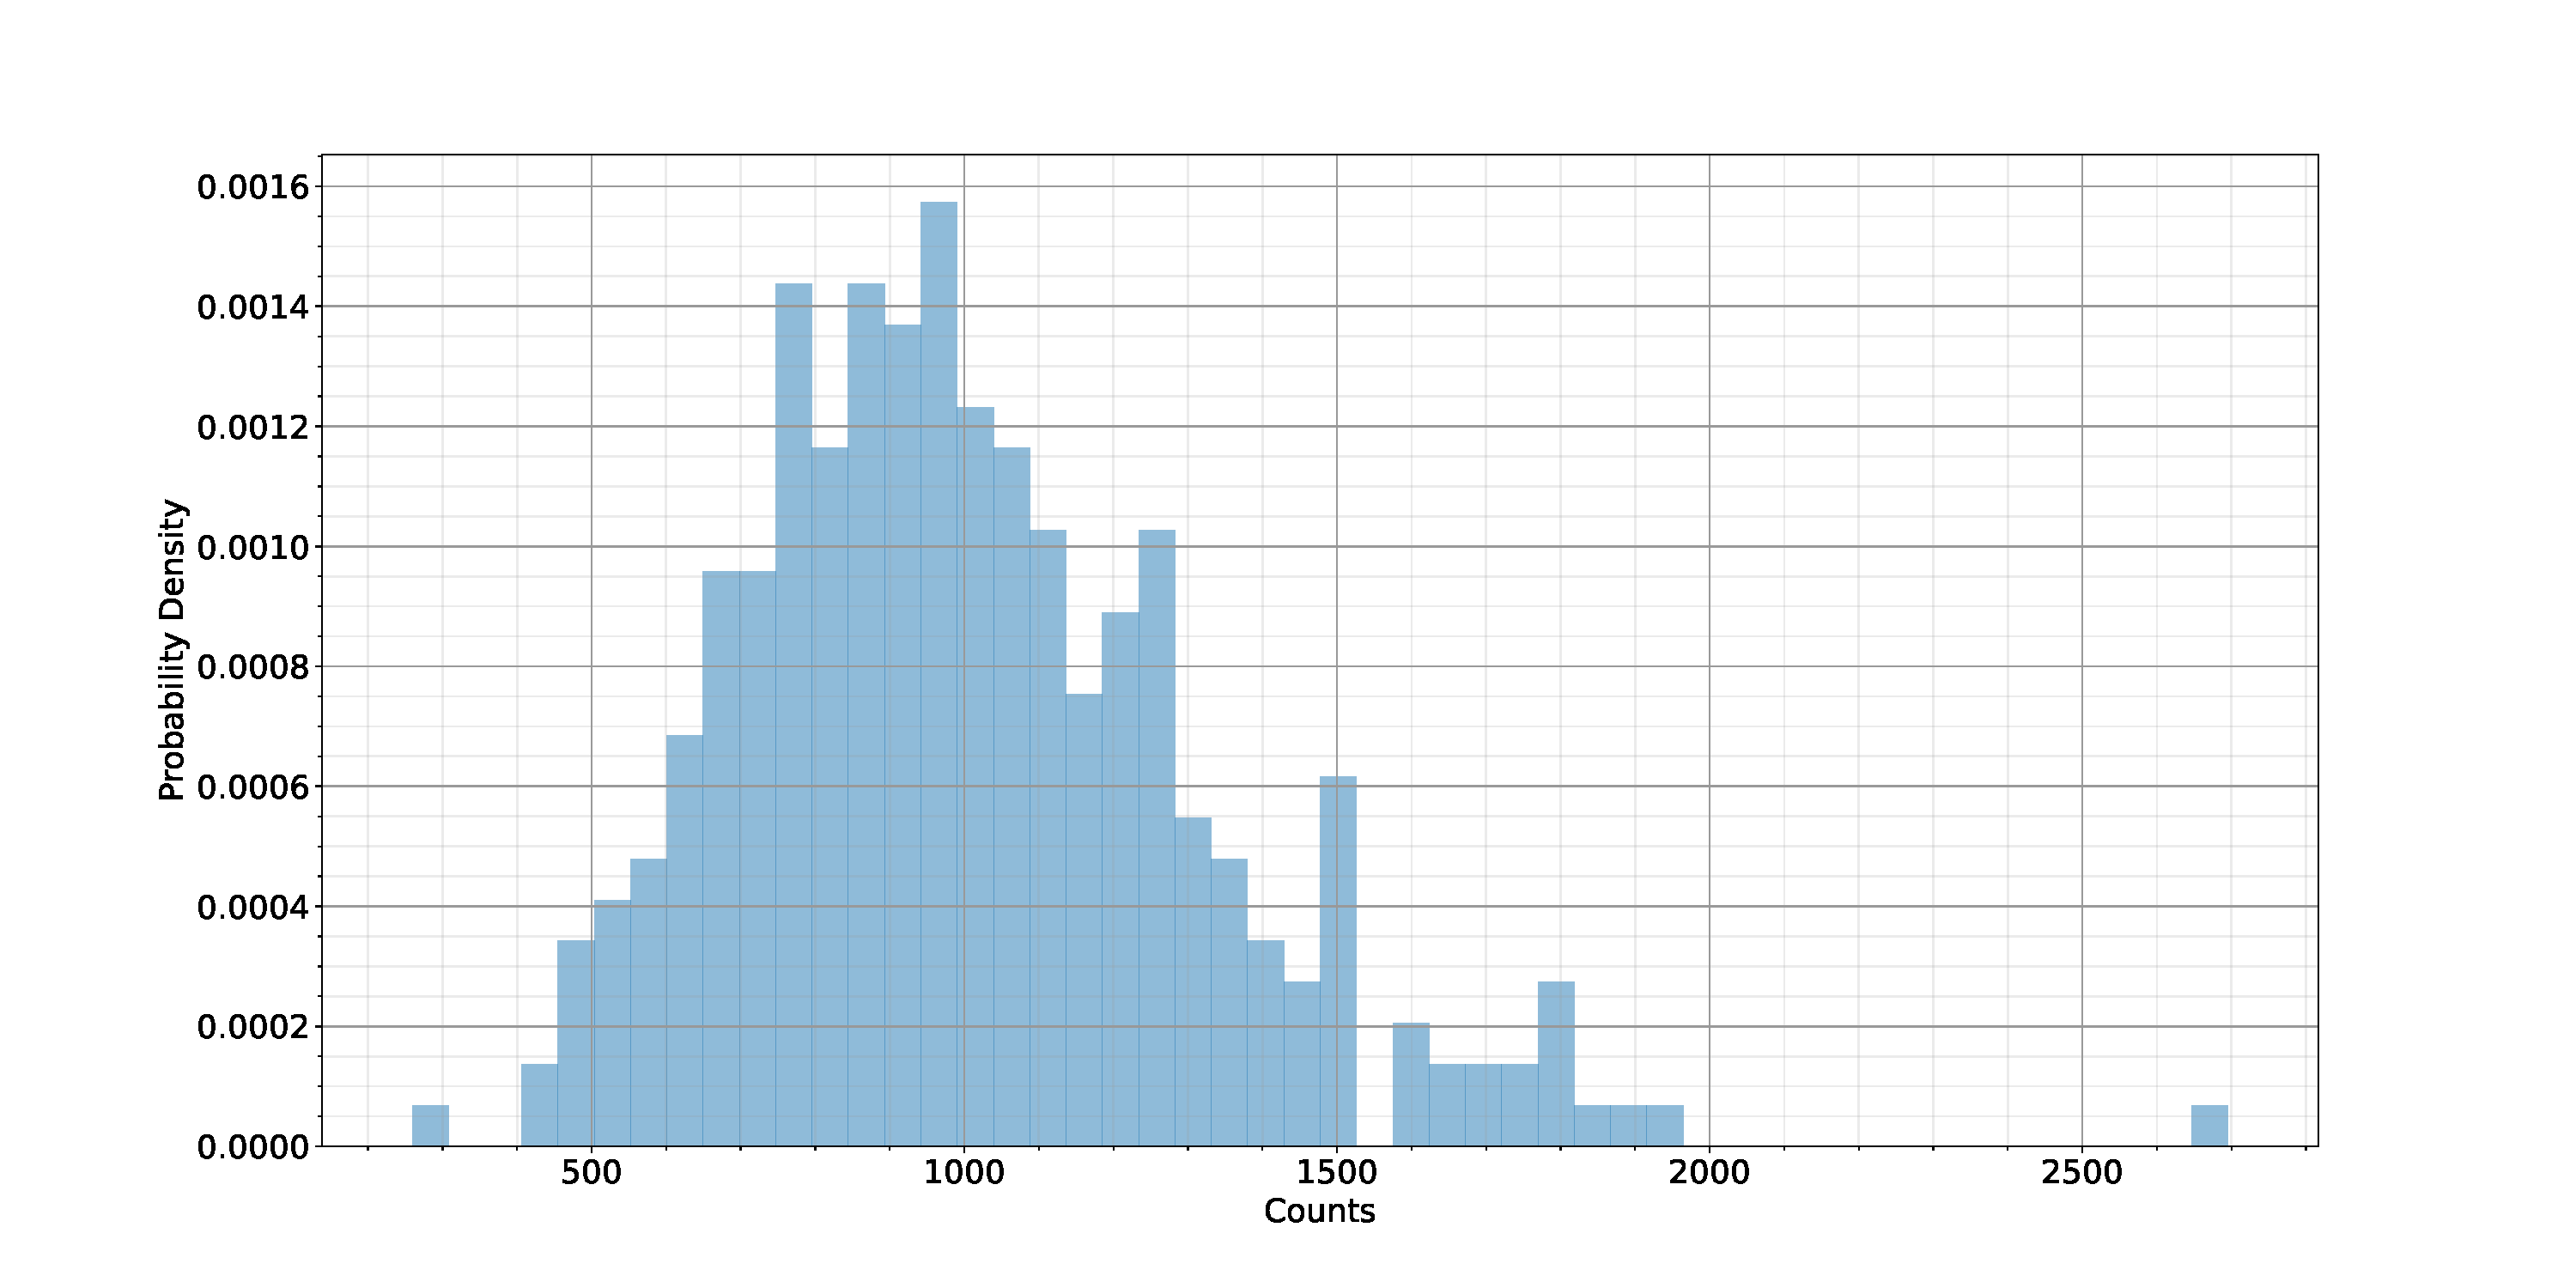
\includegraphics[width = 1\textwidth]{figures/count_hist.pdf}
		\caption{A probability density histogram for the sample of $300$ data points considered in the numerical example. The data are event counts drawn from ($300$) Poisson distributions with ($300$) rate parameters drawn from a gamma distribution with $\alpha = 10$ and $\beta =  0.01$.}
		\label{fig:q1}
	\end{figure}
	
	\begin{table}[h]
		\centering
		\begin{tabular}{|c|c|c|}
			\hline
			\multicolumn{1}{|c|}{Approximation} & \multicolumn{1}{c|}{$\mathbb{E}[x|y,I]$} & \multicolumn{1}{c|}{$\sqrt{\text{Var}[x|y,I]}$} \\
			\hline\hline
			Simple Poisson theoretical & $1008.9$ & $31.8$ \\
			Simple Poisson pymc & $1008.5$ & $31.8$ \\
			\hline
			Advanced Poisson pymc & $1008.7$ & $324.1$ \\
			\hline
			Normal theoretical & $1008.9$ & $321.3$\\
			Normal pymc & $1007.5$ & $322.2$\\
			\hline
		\end{tabular}
		\caption{Equation \eqref{eq:mean_var} computed by each of the three approximations considered here.}
		\label{tab:1}
	\end{table}
	
	\begin{figure}[H]
		\centering
		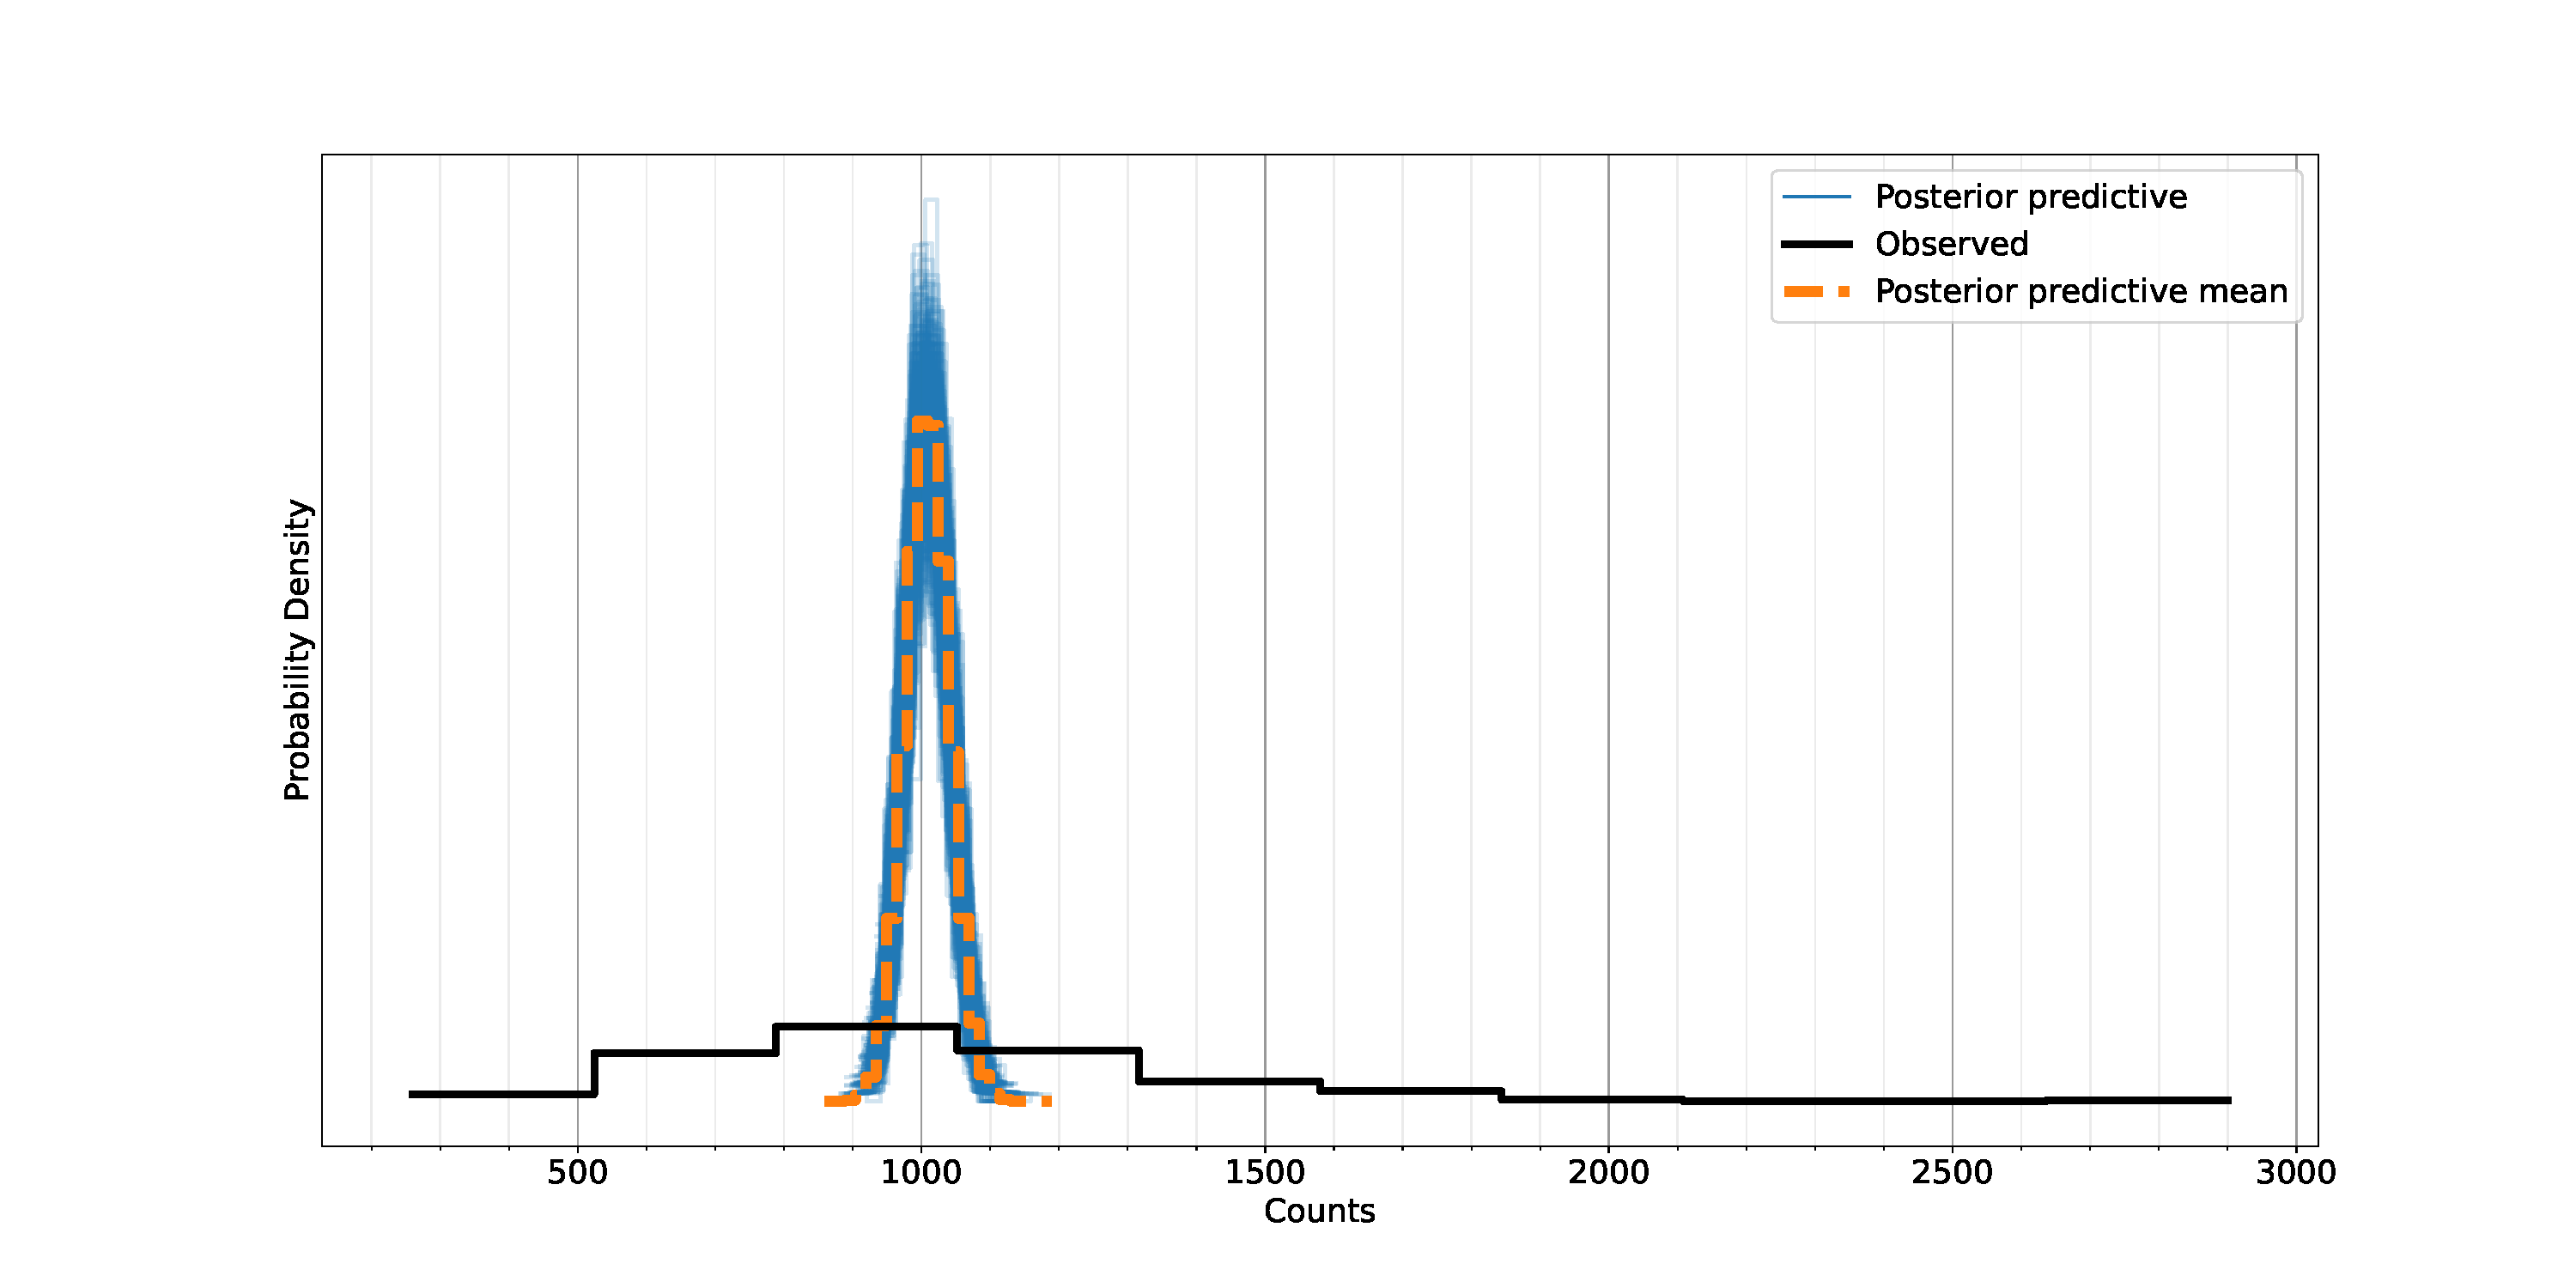
\includegraphics[width = 0.8\textwidth]{figures/pymc_poisson.pdf}
		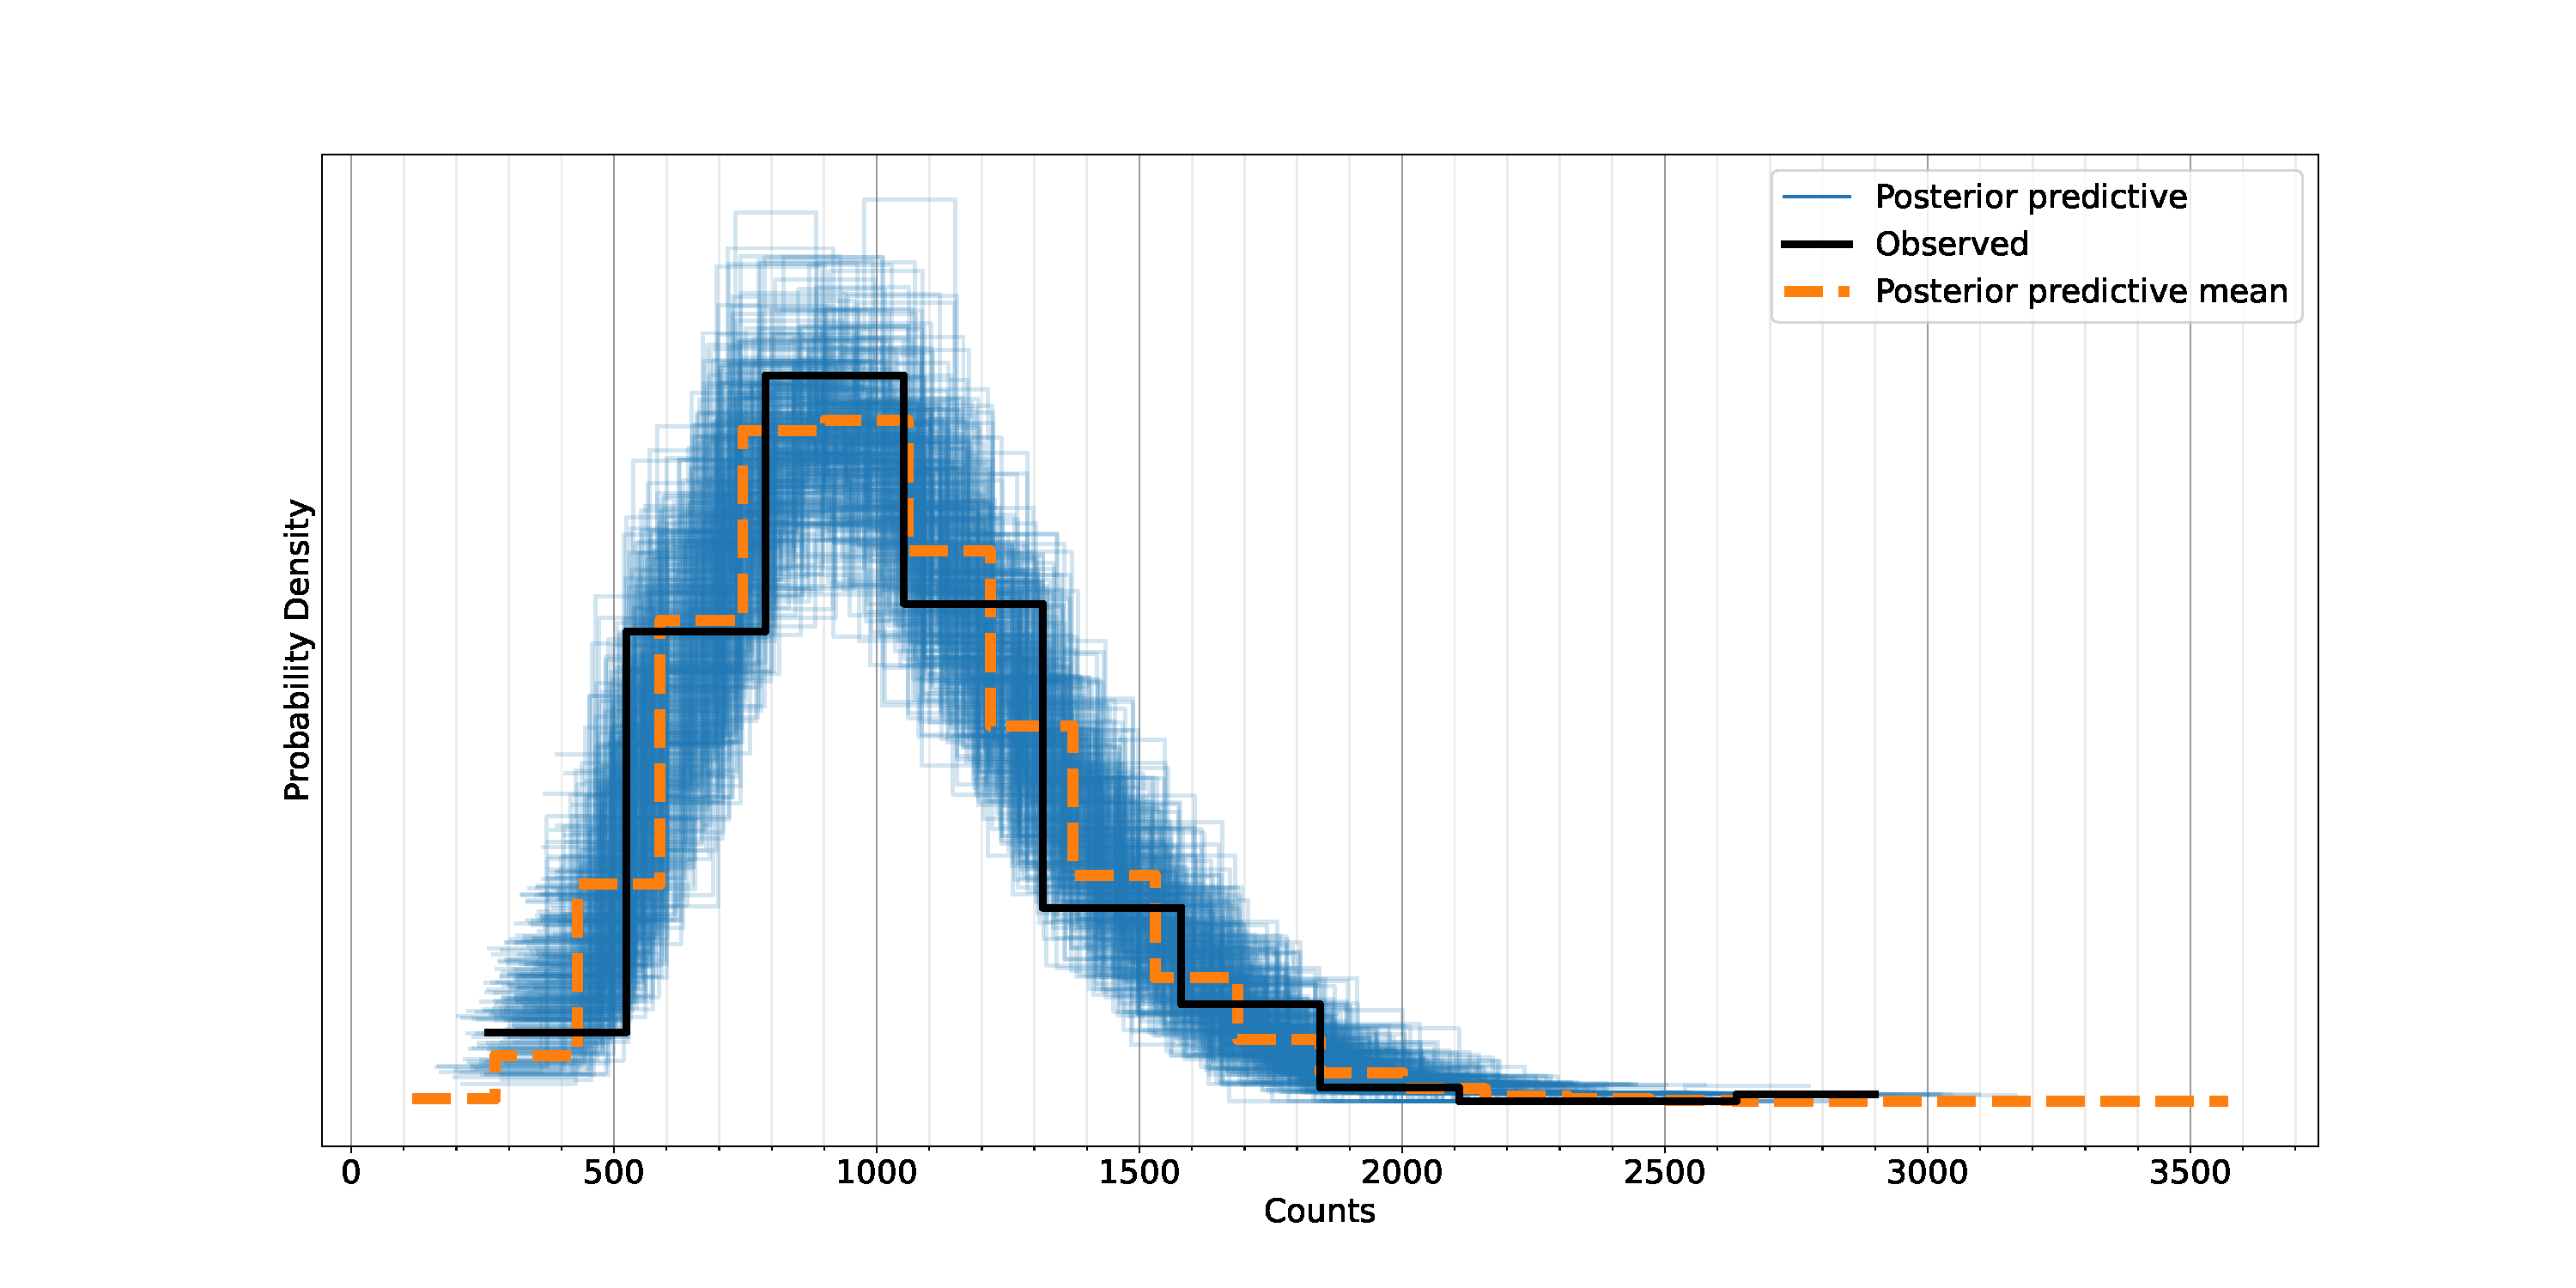
\includegraphics[width = 0.8\textwidth]{figures/pymc_negbin.pdf}
		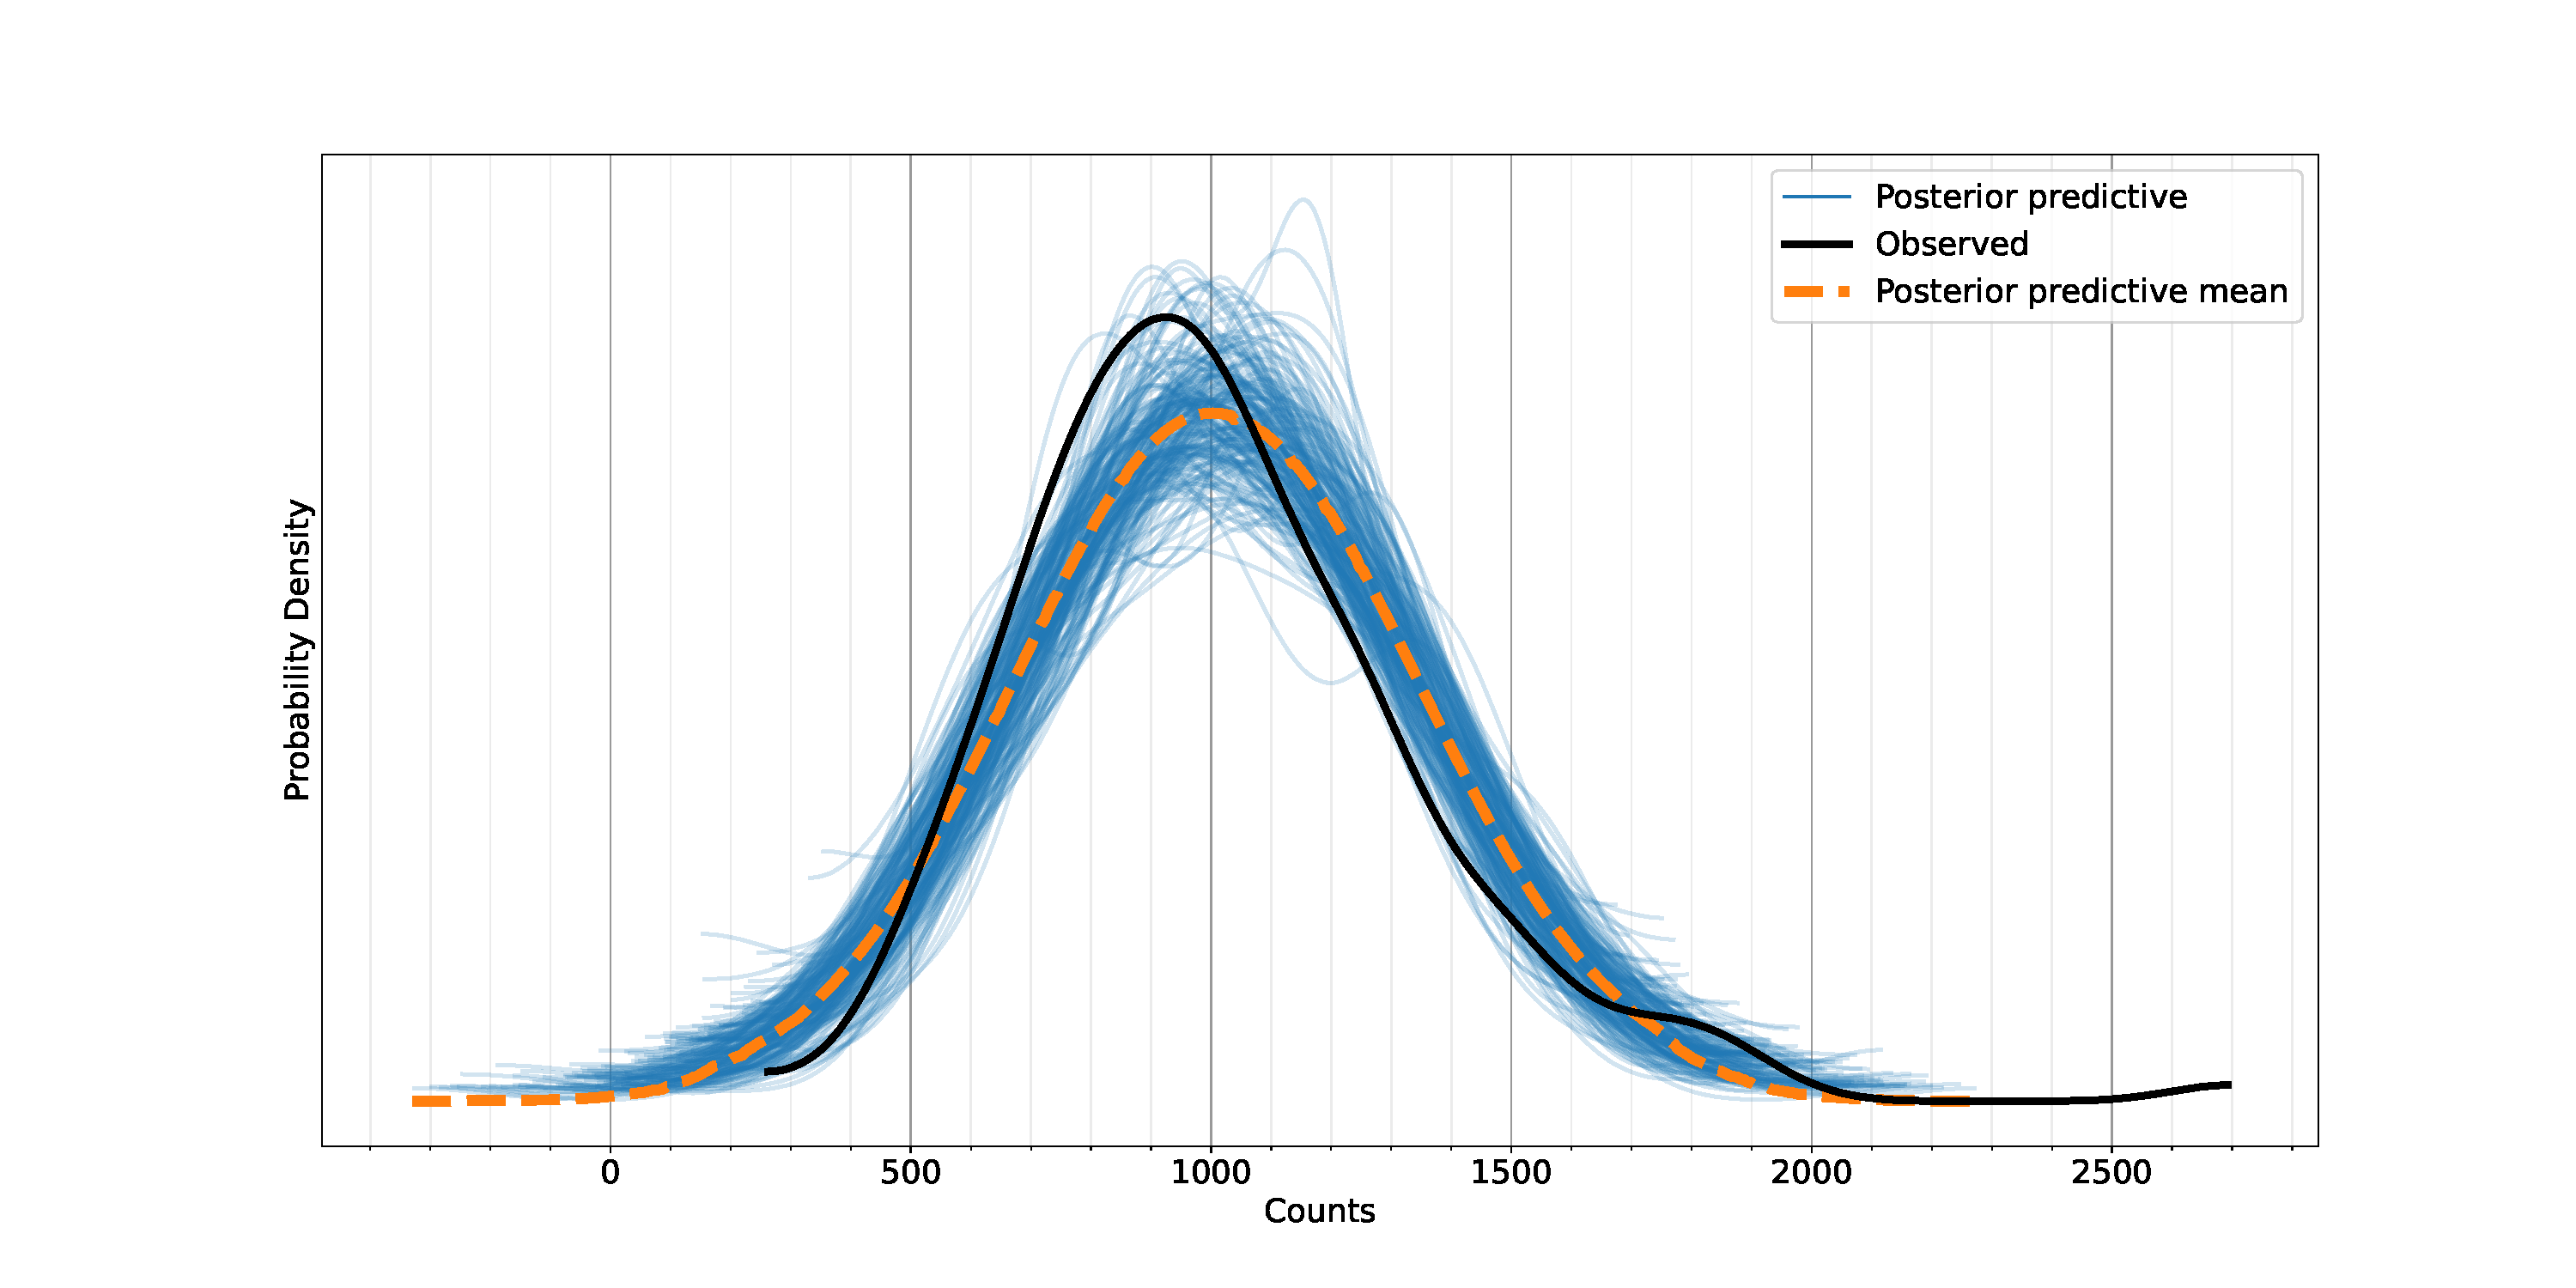
\includegraphics[width = 0.8\textwidth]{figures/pymc_normal.pdf}
		\caption{The posterior predictive distributions for the numerical example for each approximation. (top) is the simple Poisson approximation, (middle) is the advanced Poisson approximation and (bottom) is the normal approximation.}
		\label{fig:q2}
	\end{figure}
	
\end{example}



\begin{example}
	\paragraph{Setup:} Consider a farmer who wishes to retire and therefore would like to sell their set of live animals. For simplicity, assume that animals make up a simple group and a given person can either be interested in purchasing an animal or not -- the simplfication consist of not differentiating between different animal types. In order to sell their animals, the farmer needs to contact people with a sale in mind. For simplicity, the contact will be assumed to be via a telephone call only. The farmer can call (or not) with the intent to sell an animal to the recepient of the call. The recepient of the call can (or not) be interesed in purchasing an animal (Natures decision). Let $\Omega_U$ denote the set of the farmers actions and $\Omega_S$ the set of Natures actions, then
	\begin{equation}
		\begin{split}
			\Omega_U &= \{u_1 = \text{call}, u_2 = \text{don't call}\},\\
			\Omega_S &= \{s_1 = \text{interested}, s_2 = \text{not interested}\}.
		\end{split}
	\end{equation}
	A nuisance for the contacted people is associated to the call which is represented by the abstract monetary loss, $\lambda\in \mathbb{R}^+$. The degree to which people are annoyed by a sales call is independent in general and the monetary loss represents the average animosity generated and the associated moneraty loss connected to a worsened reputation. Aside from the nuisance associated with a sales call, there is also a moneraty reward for a successfull sale, $\psi$.	If the farmer cannot sell his animals, he will have them terminated with no associated cost in order not to spend additional time or money on them. Given these assumptions, the cost function can be represented by the matrix
	\begin{center}
		\begin{tabular}{  c  c  c }
			& $s_1=$ Interested & $s_2=$ Not interested  \\
			\cline{2-3}
			$u_1 =$ Call& \multicolumn{1}{|l}{$\lambda-\psi$} &\multicolumn{1}{l|}{$\lambda$}  \\
			$u_2=$ Don't call& \multicolumn{1}{|l}{$0$} & \multicolumn{1}{l|}{0} \\
			\cline{2-3}
		\end{tabular}
	\end{center}
	The farmer has available to them observations $X=x$ that contain information regarding the decesion Nature is going to make, $S=s$. The farmer also have a collection of past observations and resulting decisions of Nature, i.e. $D= \{(X=x_1,S=s_1),(X=x_2,S=s_2),\dots (X=x_n,S=s_n)\}= D_s\times D_s$. 
	
	\paragraph{Optimal decision rule:} The optimal decision for the farmer to call the $i$'th person can then be written viz
	\begin{equation}
		U^*(x) = \arg\min_{U(x)} \mathbb{E}_{S|X}[C(U(x), S)|X=x,D,I],
	\end{equation}
	where
	\begin{equation}
		\mathbb{E}_{S|X}[C(U(x), S)|X=x,D,I] = \sum_{s\in \mathbb{S}} C(U(x),s) p(S=s|X=x,D,I).
	\end{equation}
	Writing out the conditional expectation
	\begin{equation}
		\begin{split}
			\mathbb{E}[C(u_1, S)] & = \sum_sC(u_1,s)p(s)\\
			& = C(u_1,s_1)p(s_1|x,D,I) + C(u_1,s_2)p(s_2|x,D,I)\\
			& = (\lambda-\psi)p(s_1|x,D,I) + \lambda_i p(s_2|x,D,I),\\
			\mathbb{E}[C(u_2, S)] & = \sum_sC(u_2,s)p(s|x,D,I)\\
			& = C(u_2,s_1)p(s_1|x,D,I) + C(u_2,s_2)p(s_2|x,D,I),\\
			&=0
		\end{split}
	\end{equation}
	where the notation has been compressed to fit the equations to the page. The optimal decision rule $U^*(x)$ can be implicitly specified as picking $u_1$ (call) iff $\mathbb{E}_{S|X}[C(u_1, S)|x,D,I]<\mathbb{E}_{S|X}[C(u_2, S)|x,D,I]$, corresponding to picking $u_1$ (call) iff
	\begin{equation}
		(\lambda-\psi)p(S= s_1|x,D,I) + \lambda p(S= s_2|x,D,I) <0
	\end{equation}
	Since $p(S= s_1|x,D,I) +p(S= s_2|x,D,I) = 1$
	\begin{equation}
		\frac{\lambda}{\psi} < p(S= s_1|x,D,I)
		\label{eq:decision_rule}
	\end{equation}
	meaning the farmer should call (action $u_1$) iff the probability for the recepient of the call to be interested in at least one animal is larger than the penalty of calling divided by the gain of calling. 
	
	\paragraph{The Probability:} \EQref{eq:decision_rule} implicitly specify the decision rule for the farmer. $\lambda,\psi$ is assumed specified, so only the probability $p(S= s_1|x,D,I)$ remain to be specified. Suppose now a model, $f: \Omega_W\times \Omega_X\mapsto[0,1]$, with associated parameters $w\in \Omega_W$, that estimates Nature's actions $S$ based on observed data $X$ is introduced. Using marginalization and assuming independence 
	\begin{equation}
		\begin{split}
			p(S= s|x,D,I) &= \int p(S= s,w|x,D,I) dw \\
			& = \int p(S= s|x,w,D,I)  p(w|x,D,I)dw \\
			& = \int p(S= s|x,w,I)  p(w|D,I)dw. \\
		\end{split}
		\label{eq:q5a}
	\end{equation}
	Combining \EQref{eq:q5a} and \EQref{f_dist2}
	\begin{equation}
		\begin{split}
			p(S= s|x,D,I) & = \int f_{S = s}(w,x)  p(w|D,I)dw \\
			& = \mathbb{E}[f_{S = s}(w,x)|D,I].\\
		\end{split}
	\end{equation}
	From Bayes theorem \index{Bayes theorem}
	\begin{equation}
		p(w|D,I) =\frac{p(D_s|D_x,w,I)p(w|D_x,I)}{p(D_s|D_x,I)},
	\end{equation}
	where $p(w|D_x,I) = p(w|I)$. Assuming the distribution over $w$ is normally distributed with zero mean and a precision described by a hyperparameter, $\lambda$, 
	\begin{equation}
		p(w|I) = \int p(w|\lambda,I)p(\lambda|I)d\lambda.
		\label{eq:lambda}
	\end{equation}
	The precision is constructed as a wide gamma distribution so as to approximate an objective prior
	\begin{equation}
		p(w|\lambda,I)p(\lambda|I)
		= \prod_{q=1}^{\tilde{n}} \frac{\lambda_q^\frac{n_q}{2}}{(2\pi)^\frac{n_q}{2}}e^{-\frac{\lambda_q}{2}\sum_{l=1}^{n_q}w_l^2}\frac{\beta_q^{\alpha_q}}{\Gamma(\alpha_q)}\lambda_q^{\alpha_q-1}e^{-\beta_q \lambda_q}
		\label{eq:priora}
	\end{equation}
	Assuming the past actions of Nature are independent and identically distributed, the likelihood can be written 
	\begin{equation}
		\begin{split}
			p(D_s|D_x,w,I) &=\prod_{i=1}^{n}p(S = s_i|X = x_i,w,I)\\
			&=\prod_{i=1}^{n}f_{s_i}(w,x_i).\\
		\end{split}
		\label{lika}
	\end{equation}
	Aside from the specification of the model $f$, $p(S= s|x,D,I)$ is at this point fully specified and can be approximated by HMC similarly to the regression case. In this case, the model can be represented by the Hamiltonian 
	\begin{equation}
		H \equiv  \sum_{q}\sum_{l}\frac{p_{l}^2}{2m_{l}}-\ln(p(w,\lambda|D,I))+const
		\label{ham3a}
	\end{equation}
	where
	\begin{equation}
		p(w|D,I) = \int d\lambda p(w,\lambda|D,I).
	\end{equation}
	Using \EQref{eq:q5a}-\EQref{lika} in \EQref{ham3a} yields the Hamiltonian
	\begin{equation}
		\begin{split}
			H&=\sum_{q=1}^{\tilde{n}}\sum_{l=1}^{n_q}\frac{p_{l}^2}{2m_{l}}-\sum_{i=1}^{n}\ln(f_{s_i}(w,x_i))+\text{const}\\
			&\quad+\sum_{q=1}^{\tilde{n}}\bigg(\ln(\Gamma(\alpha_q))-\alpha_q\ln(\beta_q)+(1-\alpha_q)\ln(\lambda_q)+\beta_q\lambda_q\\
			&\qquad \qquad+\frac{n_q}{2}(\ln(2\pi)-\ln(\lambda_q))+\frac{\lambda_q}{2}\sum_{l=1}^{n_q}w_l^2\bigg)\\
		\end{split}.
		\label{ham2a}
	\end{equation}
	
	\paragraph{Simple model:} Let
	\begin{equation}
		f_{S = s}(w,x_i) = \frac{e^{b_s+\sum_{q}a_{sq}x_{iq}}}{\sum_{k\in \mathbb{S}}e^{b_k+\sum_{q}a_{kq}x_{iq}}},
		\label{eq:f1}
	\end{equation}
	where $w = \{b,a\}$.
	
	\paragraph{Manual HMC:}	The Hamiltonian is given by
	\begin{equation}
		\begin{split}
			H&=\sum_{q=1}^{2}\sum_{l=1}^{2}\frac{p_{ql}^2}{2m_{ql}}-\sum_{i=1}^{n}\ln(f_{s_i}(w,x_i))\\
			&\quad+\ln(\Gamma(\alpha_a))-\alpha_a\ln(\beta_a)+(1-\alpha_a)\ln(\lambda_a)+\beta_a\lambda_a\\
			&\qquad \qquad+\frac{1}{2}(\ln(2\pi)-\ln(\lambda_a))+\frac{\lambda_a}{2}\sum_{j,q}a_{jq}^2\\
			&\quad+\ln(\Gamma(\alpha_b))-\alpha_b\ln(\beta_b)+(1-\alpha_b)\ln(\lambda_b)+\beta_b\lambda_b\\
			&\qquad \qquad+\frac{1}{2}(\ln(2\pi)-\ln(\lambda_b))+\frac{\lambda_b}{2}\sum_{j}b_j^2\\
		\end{split}
	\end{equation}
	$\lambda_j$ is positive definite. In order to uphold this numerically, let $\lambda_j = e^{\tau_j}$. When making this transformation, the integration measure of \EQref{eq:lambda} has to be transformed as well. This proceeds viz
	\begin{equation}
		d\lambda_j = \lambda_jd\tau_j,
	\end{equation}
	meaning effectively $\lambda_j$ is multiplied on $p(w,\lambda|D,I)$ such that $H \rightarrow H-\ln(\lambda_j)$. This means
	\begin{equation}
		(1-\alpha_j)\ln(\lambda_j)\in H \Rightarrow -\alpha_j \ln(\lambda_j).
	\end{equation}
	Additionally, it is convenient to pick out the $s_i$ via a one-hot target vector such that
	\begin{equation}
		\begin{split}
			H&=\sum_{q=1}^{2}\sum_{l=1}^{2}\frac{p_{ql}^2}{2m_{ql}}-\sum_{j\in \mathbb{S}}\sum_{i=1}^{n}s_{ij}\ln(f_{j}(w,x_i))\\
			&\quad+\ln(\Gamma(\alpha_a))-\alpha_a\ln(\beta_a)-\alpha_a\tau_a+\beta_ae^{\tau_a}\\
			&\qquad \qquad+\frac{1}{2}(\ln(2\pi)-\tau_a)+\frac{e^{\tau_a}}{2}\sum_{j,q}a_{jq}^2\\
			&\quad+\ln(\Gamma(\alpha_b))-\alpha_b\ln(\beta_b)-\alpha_b\tau_b+\beta_be^{\tau_b}\\
			&\qquad \qquad+\frac{1}{2}(\ln(2\pi)-\tau_b)+\frac{e^{\tau_b}}{2}\sum_{j}b_j^2\\
		\end{split}
	\end{equation}
	
	The derivatives are needed for the HMC algorithm
	\begin{equation}
		\frac{\partial H}{\partial a_{ml}} = -\sum_{i,j}\frac{s_{ij}}{f_{ij}}\frac{\partial f_{ij}}{\partial a_{ml}}+e^{\tau_a}a_{ml},\\
	\end{equation}
	\begin{equation}
		\begin{split}
			\frac{\partial f_{ij}}{\partial a_{ml}} & = \frac{e^{b_j+\sum_{q_1}a_{jq_1}x_{iq_1}}}{\sum_{k\in \mathbb{S}}e^{b_k+\sum_{q_2}a_{kq_2}x_{iq_2}}}\sum_{q_3}\delta_{jm}\delta_{q_3l}x_{iq_3}\\
			&\qquad-\frac{e^{b_j+\sum_{q_4}a_{jq_4}x_{iq_4}}}{(\sum_{k\in \mathbb{S}}e^{b_k+\sum_{q_5}a_{kq_5}x_{iq_5}})^2}\sum_{k'\in \mathbb{S}}e^{b_{k'}+\sum_{q_6}a_{k'q_6}x_{iq_6}}\sum_{q_7}\delta_{k'm}\delta_{q_7l}x_{iq_7}\\
			& = f_{ij}\delta_{jm}x_{il}- f_{ij}f_{im}x_{il}
		\end{split}
	\end{equation}
	where it has been used that
	\begin{equation}
		\frac{\partial a_{jq_3}}{\partial a_{ml}} = \delta_{jm}\delta_{q_3l}
	\end{equation}
	
	\begin{equation}
		\begin{split}
			\frac{\partial H}{\partial a_{ml}} &= -\sum_{i,j}\frac{s_{ij}}{f_{ij}}(f_{ij}\delta_{jm}x_{il}- f_{ij}f_{im}x_{il})+e^{\tau_a}a_{ml}\\
			& = \sum_ix_{il}(f_{im}-s_{im})+e^{\tau_a}a_m\\
		\end{split}
	\end{equation}
	\begin{equation}
		\frac{\partial H}{\partial b_m} = \sum_i(f_{im}-s_{im})+e^{\tau_b}b_m.
	\end{equation}
	\begin{equation}
		\frac{\partial H}{\partial \tau_m} = -\alpha_m+\beta_me^{\tau_m}-\frac{1}{2}+\frac{e^{\tau_m}}{2}\sum_jm_j^2.
	\end{equation}
	
	The masses for the HMC algorithm can be set by approximating the second order derivatives as fixed. Let
	\begin{equation}
		\begin{split}
			\frac{\partial^2 H}{\partial a_{ml}^2} &= \sum_ix_{il}\frac{\partial f_{im}}{\partial a_{ml}}+e^{\tau_a}\\
			& =\sum_ix_{il}^2f_{im}( 1- f_{im})+e^{\tau_a}\\
		\end{split}
	\end{equation}
	then taking $x_{il}^2\sim 1, f_{im}\sim \frac{1}{2}$ and any parameter $\sim 0$, meaning $e^{\tau_a} \sim 1$ yield the mass approximation
	\begin{equation}
		\begin{split}
			m_{ml}^{(a)} &\sim \frac{\partial^2 H}{\partial a_{ml}^2}\bigg|_{\text{fixed approximation}}\\
			& \sim N\cdot 1^2\cdot \frac{1}{2}(1-\frac{1}{2})+1\\
			&=\frac{N}{4} +1,
		\end{split}
	\end{equation}
	where $N$ is the number of data samples in $D_x$. Similarly
	\begin{equation}
		\begin{split}
			\frac{\partial^2 H}{\partial b_m^2} &= \sum_i\frac{\partial f_{im}}{\partial a_{ml}}+e^{\tau_b}\\
			& =\sum_if_{im}( 1- f_{im})+e^{\tau_b},
		\end{split}
	\end{equation}
	meaning (since $x_{il}^2\sim 1$)
	\begin{equation}
		\begin{split}
			m_{ml}^{(a)} &\sim \frac{\partial^2 H}{\partial b_{m}^2}\bigg|_{\text{fixed approximation}}\\
			& m_{ml}^{(b)}.
		\end{split}
	\end{equation}
	The precision parameter
	\begin{equation}
		\frac{\partial^2 H}{\partial \tau_q^2} = \beta_qe^{\tau_q}+\frac{e^{\tau_q}}{2}\sum_jq_j^2.
	\end{equation}
	Take $\beta_q = 3$, then
	\begin{equation}
		\begin{split}
			m_{q}^{(\tau)} &\sim \frac{\partial^2 H}{\partial \tau_{q}^2}\bigg|_{\text{fixed approximation}}\\
			&\sim 3.
		\end{split}
	\end{equation}
	
	
	
	
	\paragraph{Data:} Take $x=(\text{area},\text{number of animals})^T$ and $s=$ 2d one-hot vector, with $\dim(D)=1000$. $D$ is split into two sets $D^{(\text{training})}$ and $D^{(\text{test})}$, with $\dim(D^{(\text{training})})=\gamma\dim(D)$ and $\dim(D^{(\text{test})})=(1-\gamma)\dim(D)$ and $\gamma=0.6$. $D^{(\text{training})}$ will be used to train the model and $D^{(\text{test})}$ to evaluate the quality of the trained model. The underlying truth of Nature (unbeknownst to the model) is that an animal will be purchased iff
	\begin{equation}
		\text{total area}- 3.2\cdot\text{number of animals}\geq 3.2.
		\label{eq:nature}
	\end{equation}
	
	\paragraph{Training:} Using $D^{(\text{training})}$ as input, the algorithms the algorithms are trained for $2000$ iterations. The first $500$ iterations are taken as burn in to be conservative. The coefficients, $w$, for iterations $[500,2000]$ are used to make a model prediction viz
	\begin{equation}
		p(S= s|x,D,I)=\frac{1}{1500}\sum_{i=500}^{2000}f(w_i,x)
	\end{equation}
	The accuracy of the modeled probabilities can be gauged by considering the case where $\psi=2\lambda$ such that the decision rule (\EQref{eq:decision_rule}) becomes
	\begin{equation}
		\frac{1}{2} < p(S= s_1|x,D,I),
		\label{eq:decision_rule2}
	\end{equation}
	and the classification is driven by the probabilities alone. 
	
	
	\paragraph{PyMC HMC Algorithm:} PyMC is a probabilistic programming library for Python that allows users to build Bayesian models with a Python API and fit them using Markov Chain Monte Carlo methods \href{https://www.pymc.io/welcome.html}{PyMC link}. Using this API it is possible to create, train and test a PyMC-equivalent of the model described in the previous sections. The general approach to building a model using PyMC consists of stating the data generating process, specifying a likelihood, and related prior distributions for any parameters involved. While modeling the data generating process and framing the statistical problem correctly are never completely trivial and require some effort from the user it is rather straight forward to perform the Markov Chain Monte Carlo sampling with PyMC. The user do not need to do any calculations related to the Hamiltonian Monte Carlo method nor do they need to specifically handle any integrals. In addition, there is a range of predefined probability distributions both discrete and continuous readily available in the library such as the Gamma (figure \ref{fig:gamma}) and Normal distribution used for modeling the priors.
	\begin{figure}[H]
		\centering
		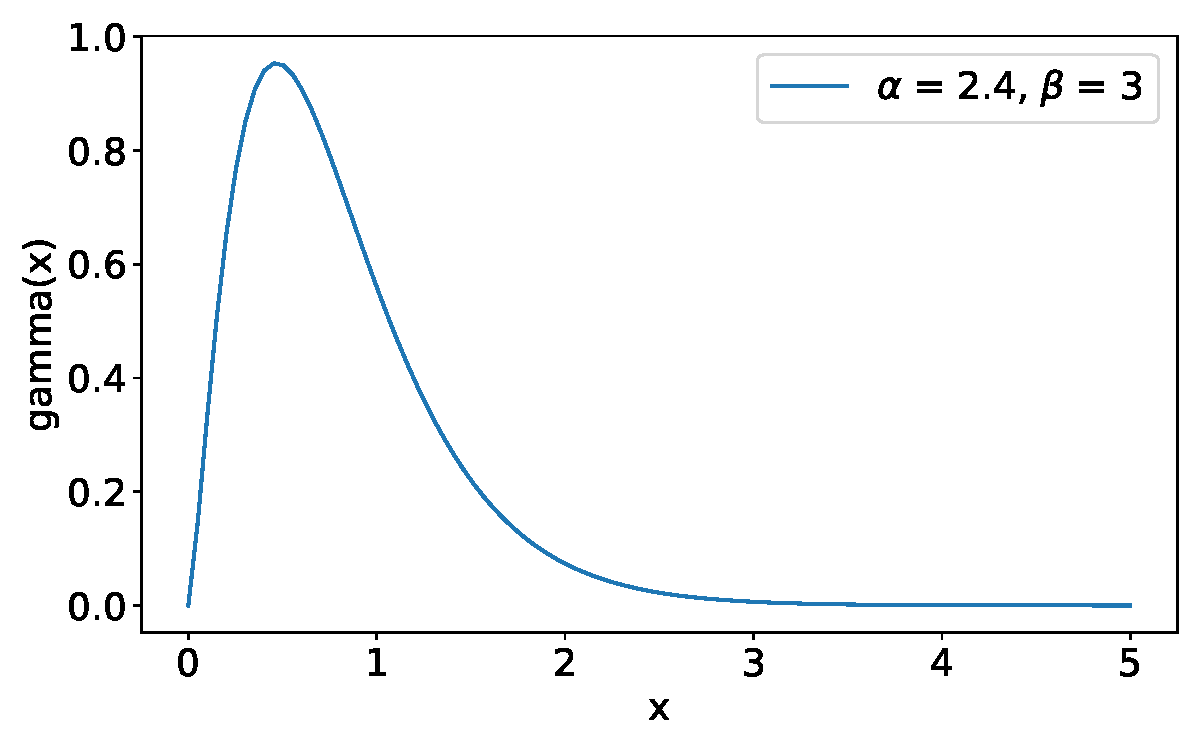
\includegraphics[width = 1\textwidth]{figures/gamma_dist.pdf}
		\caption{Plot of Gamma probability distribution used as priors for the precision parameters in Normal distributions.}
		\label{fig:gamma}
	\end{figure}
	The python code in \algref{algo:pymc_model} shows how the simple model can be declared using PyMC. All models in PyMC are declared using a "with pm.Model() as modelname"-statement, where pm is the abbreviated form of the PyMC package. Within this statement at range of random variables, data and their relations can be declared. The syntax for declaring a random variable by its probability distribution (such as pm.Normal) is to pass a name for the random variable as a string for the first argument. The rest of the arguments are typically values for the parameters specific to the distribution. PyMC random variables can often be used for stating parameters in other random variables forming a hierarchy of distributions as is the case for the precision variables used to model the variance for the normally distributed parameters a and b (see \EQref{eq:f1}) with zero mean. In the code example, these parameters are then combined deterministically with $D_x$ to constitute the data generating process of the simple model. $D_x$ is declared as a PyMC mutable object so that it will be possible later to change the values to generate predictions. As a last step the likelihood is declared. In PyMC this is the step where the relationship between the observed conditional ($D_s$) data and parameters is stated. As the output is the probabilities for the two classes a Multinomial distribution with the number of independent trials (n) equal to 1 is used as the likelihood. 
	
	\begin{algorithm}[H]
		\caption{PyMC Python Code}
		\begin{python}
			import pymc as pm
			import numpy as np
			with pm.Model() as classifier_model:
			covars = pm.MutableData('covars',data_x_training) 
			# Priors for precision
			precision_a = pm.Gamma('precision_a', alpha=2.4, beta=3)
			precision_b = pm.Gamma('precision_b', alpha=2.4, beta=3)
			# Priors for parameters
			param_a = pm.Normal('param_a', 
			0, 
			sigma=1/np.sqrt(precision_a),
			shape=(2,2))
			param_b = pm.Normal('param_b', 
			0, 
			sigma=1/np.sqrt(precision_b),
			shape=(2,))
			# Data generating process
			T = pm.Deterministic('T', pm.Math.exp(param_b + pm.math.dot(covars, param_a.T)))
			class_conditional_probability = pm.Deterministic('class_conditional_probability', T/T.sum(axis=1, keepdims=True))
			# Likelihood
			obs = pm.Multinomial('obs', n=1, p=class_conditional_probability, observed=data_s_training, shape=class_conditional_probability.shape)
		\end{python}
		\label{algo:pymc_model}
	\end{algorithm}
	
	
	After declaring the model it is possible to sample the posterior by calling the pm.sample() method. Burn-in can be controlled by setting the tune argument. The draw argument determines how many samples are being drawn while a number of chains can be run in parallel by setting the chains and cores (computational) arguments. 	
	\begin{algorithm}[H]
		\label{algo:posteriro}
		\caption{PyMC Posterior Python Code}
		\begin{python}
			with classifier_model:
			posterior = pm.sample(tune=512, draws=1024, chains=4, cores=4)
		\end{python}  
	\end{algorithm}
	
	Using the result of drawing samples from the distribution of model parameters (posterior) it is possible to draw from the posterior predictive distribution using the pm.sample\_posterior\_predictive() method. Without changing the input data this is equivalent to obtaining the result of applying the trained model on $D_x^{(\text{training})}$. By changing the input data to $D_x^{(\text{test})}$ using the pm.set\_data() method it is possible to obtain the posterior predictive distribution.
	
	\begin{algorithm}[H]
		\label{algo:posteriro_predictive}
		\caption{PyMC Posterior Python Code}
		\begin{python}
			with classifier_model:
			posterior_predictive = pm.sample_posterior_predictive(posterior)
			pm.set_data({'covars': data_x_test})
			posterior_predictive_test = pm.sample_posterior_predictive(posterior)
		\end{python}
	\end{algorithm}
	
	Using \EQref{eq:decision_rule2} for $D^{(\text{training})}$, the PyMC model correctly classify $598$ of $600$ data points. For $D^{(\text{test})}$, the model correctly classify $398$.
	
	\paragraph{Results: } The HMC algorithm have parameters "step\_scale" and "number\_of\_steps\_scale", which adjust the overall scale of the step lengths and number of steps in pase space. Ideally, the distance between points should be large, so that step scale should be small (what the step length is divided by should be small) and the number of steps should be large. Numerical stability only exist for step\_scale $\gtrsim 5$ (given accurate mass estimation) and thus only the number of steps remain as a variable to tune. In this study step\_scale $=10$ and number\_of\_steps\_scale $=1500$, where the latter is limited by reasonable computation time (to match approximately the pymc computation time). Given these parameters, the manual HMC algorithm misclassify a single training data point
	\begin{equation}
		x^{(\text{training})}_{\text{misclassified 1}} = \begin{pmatrix}
			3.21798365\\ 0\\
		\end{pmatrix}
		\label{eq:misclassified1_training}
	\end{equation}
	and two test data points
	\begin{equation}
		x^{(\text{test})}_{\text{misclassified 1}} = \begin{pmatrix}
			6.40501793\\ 1\\
		\end{pmatrix}, \quad x^{(\text{test})}_{\text{misclassified 2}} = \begin{pmatrix}
			9.60627827\\ 2\\
		\end{pmatrix}.
		\label{eq:misclassified1_test}
	\end{equation}
	With \EQref{eq:nature} in mind, it is clear that the misclassifications of \EQref{eq:misclassified1_training} and \EQref{eq:misclassified1_test} are close to the limit with respect to purchasing an animal.  
	
	
	The PyMC HMC Algorithm obtain misclassify two training data points; \EQref{eq:misclassified1_training} and 
	\begin{equation}
		x^{(\text{training})}_{\text{misclassified 2}} = \begin{pmatrix}
			12.80826256\\ 3\\
		\end{pmatrix}
		\label{eq:misclassified1_training2}
	\end{equation}
	and two test data points (\EQref{eq:misclassified1_test}).
	
	
	\paragraph{Summary and Discussion:} It has been shown how decision theory can be used in conjunction with statistics to make theoretically optimal decisions based on a user specified set of preferences (cost function). Using mock data, a "manual HMC algorithm" written by hand and a standard Python "PyMC HMC algorithm" have been compared. The two yield identical results on test data with the manual model yielding marginally better results on training data. Overall the performace is deemed equivalent both in terms of accuracy and computational speed. The manual HMC algorithm require the user to derive the gradients, write the sampling algorithm in Python and tune the algorith, whereas the latter only require a specification of the model via a standardized PyMC interface. Hence, from a user complexity perspective, the PyMC algorithm has a significant advantage.
\end{example}